% A LaTeX (non-official) template for ISAE projects reports
% Copyright (C) 2014 Damien Roque
% Version: 0.2
% Author: Damien Roque <damien.roque_AT_isae.fr>

\documentclass[oneside]{book}
\usepackage[utf8]{inputenc}
\usepackage[T1]{fontenc}
\usepackage[frenchb]{babel} % If you write in French
%\usepackage[english]{babel} % If you write in English
\usepackage{a4wide}
\usepackage{graphicx}
\usepackage{graphics}
\usepackage{caption}
\graphicspath{{images/}}
\usepackage{subfig}
\usepackage{tikz}
\usetikzlibrary{shapes,arrows}
\usepackage{pgfplots}
\pgfplotsset{compat=newest}
\pgfplotsset{plot coordinates/math parser=false}
\newlength\figureheight
\newlength\figurewidth
\pgfkeys{/pgf/number format/.cd,
set decimal separator={,\!},
1000 sep={\,},
}
\usepackage{ifthen}
\usepackage{ifpdf}
\usepackage{afterpage}
\ifpdf
\usepackage[pdftex]{hyperref}
\else
\usepackage{hyperref}
\fi
\usepackage{color}
\hypersetup{%
colorlinks=true,
linkcolor=black,
citecolor=black,
urlcolor=black}

\usepackage{lipsum}
\usepackage{titlesec}
\usepackage{sectsty}
\usepackage{eurosym}
\usepackage{listings}  
\usepackage{adjustbox}
\usepackage[graphicx]{realboxes}
\usepackage[backend=bibtex,sorting=none]{biblatex}

\lstset{
    extendedchars=true,
    literate=
  {á}{{\'a}}1 {é}{{\'e}}1 {í}{{\'i}}1 {ó}{{\'o}}1 {ú}{{\'u}}1
  {Á}{{\'A}}1 {É}{{\'E}}1 {Í}{{\'I}}1 {Ó}{{\'O}}1 {Ú}{{\'U}}1
  {à}{{\`a}}1 {è}{{\`e}}1 {ì}{{\`i}}1 {ò}{{\`o}}1 {ù}{{\`u}}1
  {À}{{\`A}}1 {È}{{\'E}}1 {Ì}{{\`I}}1 {Ò}{{\`O}}1 {Ù}{{\`U}}1
  {ä}{{\"a}}1 {ë}{{\"e}}1 {ï}{{\"i}}1 {ö}{{\"o}}1 {ü}{{\"u}}1
  {Ä}{{\"A}}1 {Ë}{{\"E}}1 {Ï}{{\"I}}1 {Ö}{{\"O}}1 {Ü}{{\"U}}1
  {â}{{\^a}}1 {ê}{{\^e}}1 {î}{{\^i}}1 {ô}{{\^o}}1 {û}{{\^u}}1
  {Â}{{\^A}}1 {Ê}{{\^E}}1 {Î}{{\^I}}1 {Ô}{{\^O}}1 {Û}{{\^U}}1
  {Ã}{{\~A}}1 {ã}{{\~a}}1 {Õ}{{\~O}}1 {õ}{{\~o}}1
  {œ}{{\oe}}1 {Œ}{{\OE}}1 {æ}{{\ae}}1 {Æ}{{\AE}}1 {ß}{{\ss}}1
  {ű}{{\H{u}}}1 {Ű}{{\H{U}}}1 {ő}{{\H{o}}}1 {Ő}{{\H{O}}}1
  {ç}{{\c c}}1 {Ç}{{\c C}}1 {ø}{{\o}}1 {å}{{\r a}}1 {Å}{{\r A}}1
  {€}{{\euro}}1 {£}{{\pounds}}1 {«}{{\guillemotleft}}1
  {»}{{\guillemotright}}1 {ñ}{{\~n}}1 {Ñ}{{\~N}}1 {¿}{{?`}}1,
}

\addbibresource{bibliographie.bib}




\usepackage{etoolbox}% http://ctan.org/pkg/etoolbox


\renewcommand{\contentsname}{test}

\renewcommand{\baselinestretch}{1.05}
\usepackage{fancyhdr}
\pagestyle{fancy}
\fancyfoot{}
\fancyhead[LO]{\bfseries\nouppercase{\rightmark}}
\setlength{\headheight}{15pt}

\let\headruleORIG\headrule
\renewcommand{\headrule}{\color{black} \headruleORIG}
\renewcommand{\headrulewidth}{1.0pt}
\usepackage{colortbl}
\arrayrulecolor{black}

\fancypagestyle{plain}{
  \fancyhead{}
  \fancyfoot[C]{\thepage}
  \renewcommand{\headrulewidth}{0pt}
}

\makeatletter
\def\@textbottom{\vskip \z@ \@plus 1pt}
\let\@texttop\relax
\makeatother

\makeatletter
\def\cleardoublepage{\clearpage\if@twoside \ifodd\c@page\else%
  \hbox{}%
  \thispagestyle{empty}%
  \newpage%
  \if@twocolumn\hbox{}\newpage\fi\fi\fi}
\makeatother

\usepackage{amsthm}
\usepackage{amssymb,amsmath,bbm}
\usepackage{array}
\usepackage{bm}
\usepackage{multirow}
\usepackage[footnote]{acronym}

\newenvironment{changemargin}[2]{%
\begin{list}{}{%
\setlength{\topsep}{0pt}%
\setlength{\leftmargin}{#1}%
\setlength{\rightmargin}{#2}%
\setlength{\listparindent}{\parindent}%
\setlength{\itemindent}{\parindent}%
\setlength{\parsep}{\parskip}%
}%
\item[]}{\end{list}}

\newcommand*{\SET}[1]  {\ensuremath{\mathbf{#1}}}
\newcommand*{\VEC}[1]  {\ensuremath{\boldsymbol{#1}}}
\newcommand*{\FAM}[1]  {\ensuremath{\boldsymbol{#1}}}
\newcommand*{\MAT}[1]  {\ensuremath{\boldsymbol{#1}}}
\newcommand*{\OP}[1]  {\ensuremath{\mathrm{#1}}}
\newcommand*{\NORM}[1]  {\ensuremath{\left\|#1\right\|}}
\newcommand*{\DPR}[2]  {\ensuremath{\left \langle #1,#2 \right \rangle}}
\newcommand*{\calbf}[1]  {\ensuremath{\boldsymbol{\mathcal{#1}}}}
\newcommand*{\shift}[1]  {\ensuremath{\boldsymbol{#1}}}

\newcommand{\eqdef}{\stackrel{\mathrm{def}}{=}}
\newcommand{\argmax}{\operatornamewithlimits{argmax}}
\newcommand{\argmin}{\operatornamewithlimits{argmin}}
\newcommand{\ud}{\, \mathrm{d}}
\newcommand{\vect}{\text{Vect}}
\newcommand{\sinc}{\ensuremath{\mathrm{sinc}}}
\newcommand{\esp}{\ensuremath{\mathbb{E}}}
\newcommand{\hilbert}{\ensuremath{\mathcal{H}}}
\newcommand{\fourier}{\ensuremath{\mathcal{F}}}
\newcommand{\sgn}{\text{sgn}}
\newcommand{\intTT}{\int_{-T}^{T}}
\newcommand{\intT}{\int_{-\frac{T}{2}}^{\frac{T}{2}}}
\newcommand{\intinf}{\int_{-\infty}^{+\infty}}
\newcommand{\Sh}{\ensuremath{\boldsymbol{S}}}
\newcommand{\C}{\SET{C}}
\newcommand{\R}{\SET{R}}
\newcommand{\Z}{\SET{Z}}
\newcommand{\N}{\SET{N}}
\newcommand{\K}{\SET{K}}
\newcommand{\reel}{\mathcal{R}}
\newcommand{\imag}{\mathcal{I}}
\newcommand{\cmnr}{c_{m,n}^\reel}
\newcommand{\cmni}{c_{m,n}^\imag}
\newcommand{\cnr}{c_{n}^\reel}
\newcommand{\cni}{c_{n}^\imag}
\newcommand{\tproto}{g}
\newcommand{\rproto}{\check{g}}
\newcommand{\LR}{\mathcal{L}_2(\SET{R})}
\newcommand{\LZ}{\ell_2(\SET{Z})}
\newcommand{\LZI}[1]{\ell_2(\SET{#1})}
\newcommand{\LZZ}{\ell_2(\SET{Z}^2)}
\newcommand{\diag}{\operatorname{diag}}
\newcommand{\noise}{z}
\newcommand{\Noise}{Z}
\newcommand{\filtnoise}{\zeta}
\newcommand{\tp}{g}
\newcommand{\rp}{\check{g}}
\newcommand{\TP}{G}
\newcommand{\RP}{\check{G}}
\newcommand{\dmin}{d_{\mathrm{min}}}
\newcommand{\Dmin}{D_{\mathrm{min}}}
\newcommand{\Image}{\ensuremath{\text{Im}}}
\newcommand{\Span}{\ensuremath{\text{Span}}}

\newtheoremstyle{break}
  {11pt}{11pt}%
  {\itshape}{}%
  {\bfseries}{}%
  {\newline}{}%
\theoremstyle{break}

%\theoremstyle{definition}
\newtheorem{definition}{Définition}[chapter]

%\theoremstyle{definition}
\newtheorem{theoreme}{Théorème}[chapter]

%\theoremstyle{remark}
\newtheorem{remarque}{Remarque}[chapter]

%\theoremstyle{plain}
\newtheorem{propriete}{Propriété}[chapter]
\newtheorem{exemple}{Exemple}[chapter]

\parskip=5pt
%\sloppy

\begin{document}

%%%%%%%%%%%%%%%%%%
%%% First page %%%
%%%%%%%%%%%%%%%%%%

\begin{titlepage}
\begin{center}

\begin{figure}[!tbp]
  \centering
  \begin{minipage}[b]{1\textwidth}
    \includegraphics[width=\textwidth]{parisnanterre.jpg}
  \end{minipage}
\end{figure}

\noindent

{\large Master MIAGE 2\up{ème} année}\\[0.5cm]

{\large Mémoire Nicolas Piot}\\[0.5cm]

% Title
\rule{\linewidth}{0.5mm} \\[0.4cm]
{ \huge \bfseries Comment familiariser les concepts informatiques aux enfants ? \\[0.4cm] }
\rule{\linewidth}{0.5mm} \\[1.5cm]
% Author and supervisor
\noindent
\begin{minipage}{0.4\textwidth}
  \begin{flushleft} \large
    \emph{Auteur :}\\
    Nicolas \textsc{Piot}\\
  \end{flushleft}
\end{minipage}%
\begin{minipage}{0.4\textwidth}
  \begin{flushright} \large
    \emph{Encadrant université :} \\
    M. Fabrice \textsc{Legond}\\
  \end{flushright}
\end{minipage}

\vfill

% Bottom of the page
{\large Année universitaire 2018-2019}

\end{center}
\end{titlepage}

%%%%%%%%%%%%%%%%%%%%%%%%%%%%%
%%% Non-significant pages %%%
%%%%%%%%%%%%%%%%%%%%%%%%%%%%%


\chapter*{Remerciements}

Je souhaite avant toute chose remercier les personnes qui ont contribué à la mise en oeuvre de ce mémoire.\\


Merci donc à Fabrice Legond, mon tuteur, Pascal Poizat, Bilal Ajaj pour leurs expertises leurs conseils et leurs soutiens sur mon travail.

Merci aussi à Fabien Michel ainsi qu'à Clément Lhuillier pour leurs idées qui m'ont inspiré pour certaines parties de ce mémoire.

Merci également à ma mère pour la relecture du mémoire.

J'aimerais également remercier toutes les personnes qui ont eu un rôle non direct sur ce mémoire via leurs travaux de recherches qui m'ont permis de m'inspirer et de proposer une réflexion sur ce sujet.




\makeatletter
\def\@makechapterhead#1{%
  \vspace*{50\p@}%
  {\parindent \z@ \raggedright \normalfont
    \ifnum \c@secnumdepth >\m@ne
      \if@mainmatter
        \Huge\bfseries\space\thechapter.\space
      \fi
    \fi
    \interlinepenalty\@M
    \Huge \bfseries #1\par\nobreak
    \vskip 40\p@
  }}
\makeatother

\makeatletter
% \patchcmd{<cmd>}{<search>}{<replace>}{<success>}{<failure>}
% --- Patch \chapter
\patchcmd{\@makechapterhead}{50\p@}{\chapheadtopskip}{}{}% Space from top of page to CHAPTER X
\patchcmd{\@makechapterhead}{20\p@}{\chapheadsep}{}{}% Space between CHAPTER X and CHAPTER TITLE
\patchcmd{\@makechapterhead}{40\p@}{\chapheadbelowskip}{}{}% Space between CHAPTER TITLE and text
% --- Patch \chapter*
\patchcmd{\@makeschapterhead}{50\p@}{\chapheadtopskip}{}{}% Space from top of page to CHAPTER TITLE
\patchcmd{\@makeschapterhead}{40\p@}{\chapheadbelowskip}{}{}% SPace between CHAPTER TITLE and text
\makeatother
% Set new lengths
\newlength{\chapheadtopskip}\setlength{\chapheadtopskip}{-90pt}
\newlength{\chapheadsep}\setlength{\chapheadsep}{10pt}
\newlength{\chapheadbelowskip}\setlength{\chapheadbelowskip}{10pt}

\renewcommand{\contentsname}{Sommaire}

{\small\tableofcontents}






%%%%%%%%%%%%%%%%%%%%%%%%%%%%%%%%%%%%%%%%%%%%
%%% Content of the report and references %%%
%%%%%%%%%%%%%%%%%%%%%%%%%%%%%%%%%%%%%%%%%%%%

\mainmatter
\pagestyle{fancy}
\afterpage{\cfoot{\thepage}}
\setcounter{page}{3}

\cleardoublepage



\chapter{Présentation}
\label{chap:presentation}
%\minitoc

\section{Introduction}
Il est certain que l'informatique prend une place de plus en plus importante pour tout le monde. Que ce soit pour les utilisateurs ou les concepteurs, le monde informatique se complexifie et s'élargie en différents domaines si bien qu'aujourd'hui il parait nécessaire d'avoir certaines notions, même basiques, pour mieux appréhender le monde qui nous entoure. Si nous prenons le cas français, l'informatique est enseignée pour l'instant seulement en terminale S dans une spécialité que l'élève choisit parmi d'autres spécialités (en l'occurrence la spécialité ISN : informatique et science du numérique). En mathématique, nous voyons aussi quelques notions algorithmiques basiques mais qui ne sont pas accessibles à toutes les filières. 

Toujours en France, l’Éducation nationale a annoncé la création du Capes d’informatique en 2020. \cite{3} Une décision qui consacre l’enseignement des sciences du numérique en tant que nouvelle discipline scolaire. Cette enseignement prendra effet dans un premier temps dans les lycées dans le but de sensibiliser les élèves aux concepts informatiques basiques. L'objectif n'est pas de former des ingénieurs informatiques mais de donner des notions pour que les élèves se donnent une idée concrète de l'informatique et voir si cela leur plaît.

Un nouveau problème se pose, comment aborder le sujet de l'informatique de façon ludique à des personnes qui ne sont à la base pas forcément intéressées par ce sujet ? Quelles solutions d'apprentissages peut-on mettre en place pour familiariser les enfants et adolescents aux concepts informatiques pour qu'ils comprennent mieux le monde qui nous entoure et surtout le monde de demain ? C'est ici dans ce mémoire que nous allons tenter de répondre à cette question en abordant différents concepts, en parlant premièrement de l'existant puis ensuite de solutions proposées. Nous nous attarderons sur un point vue enfance et adolescence pour englober différentes situations possibles.

C'est pour cela que dans un premier temps nous allons parler des concepts qui me semblent importants en informatique, en partant d'un cas plutôt général vers des cas plus particuliers. Nous allons aussi parler des différentes contraintes liées à la problématique. Ensuite, nous aborderons l'existant dans l'état de l'art pour le comparer et faire le lien avec mes propositions dans la partie suivante. Ces propositions seront analysées (forces et faiblesses), puis nous finirons avec les évolutions possibles et une synthèse.

\clearpage


\section{Étude et contexte du problème}
\subsection{Les concepts informatiques}
Les domaines informatiques sont nombreux. On peut penser dans un premier temps au développement et à la programmation, à la modélisation et à la conception de systèmes d'informations. Il y a également l'aspect base de données, réseaux, l'algorithmique, les commandes Unix etc... Chacun de ces domaines ont leurs spécificités et sont plus ou moins accessibles à l'apprentissage selon les âges. Il parait par exemple difficile d'apprendre à des enfants d'administrer une base de données mais nous pouvons leur inculquer des manières de réfléchir en s'écartant des conventions et surtout de façon ludique. Ce qui est important n'est pas connaître les détails d'un domaine informatique mais en appréhender les bases dans un environnement non complexe pour l'enfant ou l'adolescent. Si, de surcroît, cet environnement est familier, cela facilitera grandement les choses. Par conséquent, il semble important de trouver pour chacun de ces domaines des solutions intelligentes pour l'apprentissage et la familiarisation avec la technologie.

\subsection{Acessible aux enfants ?}
Ce qui peut être clair pour nous ne l'est pas forcément pour les autres. Cette phrase est importante quand on travaille dans l'apprentissage. Avec un sujet comme celui-ci, la première question que l'on se pose est : est-ce que apprendre des domaines informatiques à des enfants est une idée viable ? Est-ce qu'un enfant peut être sensible à un apprentissage de ces matières qui semblent à première vue compliquées ? En me fiant aux travaux de chercheurs de l'université de Canterbury en Nouvelle Zélande \cite{1} on peut déjà avoir une idée de la sensibilité des enfants à l'apprentissage de l'informatique. En l'occurrence, la première étude indique que l'apprentissage dépend fortement des outils employés et du contexte. Il est notamment important de laisser les enfants découvrir les concepts par eux même et il faut leur offrir des opportunités pour leur permettre de continuer leur apprentissage. Les chercheurs en ont défini alors des critères majoritaires permettant une meilleure introduction à la programmation et une meilleure réceptivité de l'enfant. Ici, on ne parle pas forcément de moyen pour apprendre mais plus du contexte d'apprentissage qui permet d'évoluer dans un domaine de façon efficace. Alors oui, apprendre l'informatique à des enfants c'est possible mais avant de vouloir familiariser ou sensibiliser il faut bien s'y prendre. Ce que l'on sait des résultats de cette étude et également confirmé par d'autres \cite{8} c'est qu'enseigner l'informatique aux enfants est non seulement possible mais également recommandé. Les enfants de 4 et 5 ans peuvent apprendre les fondements informatiques avant même de savoir lire et écrire. Finalement les chercheurs ont défini différents niveau d'apprentissage, de 5 à 10 ans avec peu d'abstraction il peuvent apprendre les rudiments des fonctions, variables, itérations, les structures indexés ainsi que les conditions.
Les environnements les plus appropriés pour ce genre d'apprentissage sont les "drag and drop" ou "glisser-"déposer" (Voir annexe). Avec le temps, il est possible d'apprendre entièrement ces concepts pour des enfants de 14 ans et plus.

\newpage

\subsection{Enseigner l'informatique en primaire ?}

L'informatique pour l'instant ne s'apprend pas à l'école primaire, on peut alors penser que ce n'est pas impactant de faire cela. Plus encore, l'écriture, les mathématiques ou encore l'apprentissage de la langue semblent être plus fondamentale. Les élèves ont déjà parfois des programmes assez chargés, il serait donc non convenu de leur rajouter des choses. De plus, on observe que certains élèves de primaire possèdent des lacunes en lecture et en écriture en rentrant au collège et que ainsi il est plus prioritaire de pallier ces dites lacunes plutôt que de rajouter des enseignements. \cite{4} \cite{5}

Dans le contexte de la problématique de ce mémoire, l'objectif n'est pas forcément d'instaurer des matières foncièrement informatiques à l'école primaire (même si ceci peut être par contre intéressant au lycée), mais plutôt de trouver un moyen d'introduire des concepts avec d'autres matières qui permettent une première sensibilisation de l'élève même sans savoir que ce dernier fait quelque chose qui a un rapport avec l'informatique. En connaissance de ceci, la mission est donc de se concentrer sur des moyens efficaces (soit déjà existants soit avec ma propre contribution) de familiarisation de l'informatique. Cependant, on peut aussi réfléchir au contexte d'implantation dans un milieu éducatif même en primaire.

\subsection{L'intérêt ?}

La question de l'intérêt d'apprendre ou de familiariser des enfants à l'informatique peut aussi se poser. Comme abordé légèrement dans l'introduction, apprendre des notions informatiques aux enfants leur permet de se préparer dans le monde dans lequel nous vivons aujourd'hui. Communication, éducation, banque, réseaux sociaux, sécurité, shopping, domotique... L'informatique est présente dans énormément d'aspects de note vie. 
L'apprentissage de ce domaine permet aussi de posséder de nouvelles façons de réfléchir. Algorithme, récursion, heuristique, même sans connaître ces mots les enfants peuvent appréhender les bases de ces concepts. On peut également dire que l'informatique peut être un facteur de créativité chez l'enfant liant la résolution de problèmes (jeux, animation, puzzle ...) et l'amusement. Savoir comment certaines choses fonctionnent peut aussi être intéressant (on peut par exemple penser à un jeu vidéo). Toutes ces choses font que l'intérêt est non négligeable et qu'il sera de plus en plus important avec le temps. \cite{9}

\subsection{En résumé}

L'informatique est donc un domaine à part ? La question est légitime, comme dit précédemment, cela semble être plus simple d'apprendre des additions à un enfant que de lui apprendre l'algorithmique. Pourtant, si on réfléchit bien au problème il est possible de créer des structures adaptées aux enfants en prenant par exemple un environnement ludique. L'important dans l'apprentissage va être le contexte, si l'on donne aux enfants les outils nécessaires à l'investissement dans l'apprentissage de l'informatique alors, cet apprentissage peut être semblable et surtout accessible en comparaison avec n'importe quelle autre matière. L'important est que ce soit parlant pour l'élève. On peut notamment penser à des expériences qui ont démontrées que si l'on présente un exercice comme un exercice de géométrie ou de dessins, le taux de réussite est plus élevé dans le premier cas que dans le second. \cite{6} \cite{7}

Par conséquent, si nous présentons l'informatique de façon ludique et non complexe nous pourrons avoir des résultats sûrement similaires. Mais le problème étant toujours présent, comment faire  exactement ?

%%% Local Variables: 
%%% mode: latex
%%% TeX-master: "isae-report-template"
%%% End: 

\chapter{État de l'art}
\label{chap:lestage}

\section{Introduction}

\subsection{Présentation}

Dans cette partie, nous allons étudier l'existant en rapport avec la problématique de ce mémoire. Nous nous attarderons donc sur différents domaines d'apprentissages et différentes solutions qui existent. 

Nous aborderons donc ce qui existe dans le domaine de la recherche (par exemple des expérimentations faites sur des enfants qui ont pu rendre d'un résultat interprétable  auquel en découle des hypothèses, des faits et une conclusion). Que ce soit des recherches plutôt hypothétique ou bien des cas concrets il sera alors intéressant de voir l'impact de l'apprentissage de l'informatique sur les enfants en n'oubliant pas le contexte des expériences menées. Pour être plus précis sur le contexte : avons nous à faire à des recherches sur les enfants, adolescents etc... ? Quel est le cadre et le but de la recherche exactement ? Quel environnement est utilisé ? 

Nous aborderons également ce qui existe comme solutions "immédiates". C'est à dire des programmes ou logiciels qui sont destinés aux enfants pour leur apprendre des bases de l'algorithmique ou de la programmation et que l'on peut par exemple appliquer à ses propres enfants. Ici, nous n'avons donc pas d'étude ou de résultats mais une présentation de différents outils disponibles sur le web ou autres pour se familiariser sur la programmation selon les âges. Par conséquent ceci est très accessible et ne rentre pas dans un cas scolaire.

L'éducation de l'informatique peut aussi passer par des jeux manuels ou de réflexions ou l'enfant interagit avec un environnement pour accomplir, sans le savoir, des travaux informatiques d'ordinateur (par exemple tri etc...).

Enfin nous consacrerons également une partie sur les "serious game" ou l'apprentissage avec le jeu ayant un apport pédagogique. On retrouve notamment beaucoup de serious game pour apprendre à programmer. Pour résumé simplement, on doit écrire dans ces jeux des lignes de codes pour contrôler un personnage et interagir avec un environnement virtuel.

\subsection{Les critères de comparaison}

Parmis tous les modes d'apprentissages il me paraît important de mettre pour chacun d'entre eux des critères de comparaisons récurrents. Un premier critère serait de noter l'apport pédagogique de la solution proposé (Apprend-t-on vraiment quelque chose d'utile, est-ce réutilisable dans le futur ou est-ce éphémère ?). Notamment, est-ce que l'expérience proposée par cette solution a un vrai impact sur la population qui a participé à cette dernière ?

L'efficacité de la solution semble également être un critère important. Plus précisément savoir si c'est ennuyant et si l'expérience est donc éphémère ou bien si c'est plutôt addictif en plus d'être pédagogique.

Enfin, un critère aussi est de savoir si on parle de solution qui requiert déjà d’avoir des connaissances informatiques en plus d’en apprendre de nouvelles ou est-ce que cela peut s’adresser à de parfaits néophytes ?

Aussi est-ce que la solution est accessible d'un point de vue prix ? Est-ce que des infrastructures scolaires peuvent se permettrent d'acheter les licences d'un logiciel pédagogique ou bien avons nous à faire à une solution gratuite ?

Un dernier critère pourrait aussi être la connaissance du contexte dans lequel s'inscrit cette solution : Un contexte scolaire, extra-scolaire et encadré ou bien un contexte dans un cadre personnel (par exemple expérimentation du serious game chez soi). Dans le contexte extra scolaire on peut notamment penser aux ateliers pour enfants qui visent à s'initier à la programmation créative, robot etc...

\section{L'existant}

\subsection{Découverte et enseignement}

\subsubsection{Le doodle de Google}

Dans un premier temps il me semble cohérent de parler de solutions s'adressant à des jeunes enfants et qui plus est totalement accessible c'est à dire ne nécessitant aucune base et pas forcément d'environnement scolaire. Cette idée sera développée dans les deux premières parties. 

Parlons dans un premier temps de l'algorithmique. Cette 'discipline' peut être exercée par enfants comme adultes sans même le savoir, pourtant ici on parle bien d'un domaine qui a un rapport avec l'informatique. Si nous devons définir l'algorithmique nous pourrions dire que c'est une suite d'instructions ou d'opérations mathématiques dans l'objectif de résoudre un problème. Il peut par exemple être traduit pour l'ordinateur via un langage de programmation afin de l'exécuter. Si nous prenons un exemple concret, résoudre un rubik's cube nécessite souvent l'utilisation d'algorithme, mais nous aurons l'occasion de revenir sur cette idée plus tard dans le mémoire. 

Ici en l'occurrence je ne vais pas tout de suite aborder des expérimentations scientifiques visant à produire des résultats interprétables mais des solutions existantes et facilement accessibles. En parlant d'accessibilité, le premier cas d'étude sera un doodle de Google. Par conséquent, on imagine bien que même pour les parents n'ayant aucun rattachement professionnel à l'algorithmique, ce doodle a pu être une occasion pour eux et pour leurs enfants de découvrir concrètement ce procédé.

De quoi parle-t-on ? Le Doodle du 4 décembre 2017 fêtant le cinquantième anniversaire de l'encodage accessible aux enfants. \cite{10} \cite{11}

\begin{figure}[!htb]
  \centering
  \includegraphics[width=105mm,scale=0.5]{images/nosoluce.PNG}
  \caption{Le niveau 4 du doodle}
  \label{fig:boat1}
\end{figure}

L'objectif ici est d'aider le lapin à manger toutes ses carottes en lui suggérant un chemin à prendre à l'aide de blocs de codes. Présentons plus en détail l'interface que l'on voit sur la figure 2.1 ; En bas nous avons les blocs de codes plus particulièrement la boucle en orange avec un indice '4' spécifiant que nous rentrons 4 fois dans la boucle, la flèche verte pour faire avancer le lapin et la bleu pour faire tournoyer le lapin selon la droite ou la gauche (sur la figure seulement à droite). Sur la ligne du dessus nous avons la ligne d'exécution du code où nous allons mettre nos instructions et enfin le bouton orange pour exécuter notre code. Ici nous avons donc un premier exemple de mise en place d'un algorithme en utilisant quelques notions basique comme la boucle et l'instruction. Avez vous trouvé la solution de la figure ci dessus ?

\newpage

\begin{figure}[!htb]
  \centering
  \includegraphics[width=115mm,scale=0.5]{images/soluce2.PNG}
  \caption{Solution du problème}
  \label{fig:boat1}
\end{figure}

Le problème peut paraître assez simple pour nous mais est tout nouveau pour un enfant. Il faut aussi préciser que dans le cadre de ce jeu l'introduction à la boucle arrive au niveau 4 et que donc on accompagne intelligemment l'enfant pour la résolution des niveaux. Si vous voulez vous même essayer ce doodle le lien est disponible dans la bibliographie. Les niveaux suivants introduisent d'autres concepts comme la double boucle et demandent plus de réflexions. (Voir figure 2.3)

\begin{figure}[!htb]
  \centering
  \includegraphics[width=115mm,scale=0.5]{images/soluce3.PNG}
  \caption{Niveau 5 et sa solution}
  \label{fig:boat1}
\end{figure}

Nous avons donc présenté ici une solution à la sensibilisation de l'algorithmique aux enfants. Cette dernière est ludique et accessible, l'enfant à la mainmise et la forme du jeu peut le pousser à s'investir davantage. Cependant, nous n'avons aucune donnée réelle sur l'efficacité de ce concept et l'expérience est plutôt éphémère puisque seulement 6 niveaux sont disponibles. Le doodle à été accessible 1 jour et nous n'avons pas de retour statistiques sur par exemple, est-ce que les utilisateurs ont aimé ? Quel âge avaient-ils ? Est-ce que cette expérience les a poussés à vouloir aller plus loin dans l'apprentissage de l'algorithmique ou de la programmation ? etc..

De ce fait, on ne peut pas interpréter scientifiquement et rigoureusement des hypothèses sur l'utilisation de ce doodle. Ce que l'on peut dire c'est que c'est une solution de familiarisation à l'algorithmique tant l'interface est simple et bien décrite.

\subsubsection{Le Langage Logo}

Ce que l'on peut noter par contre en partant de ce doodle, c'est que, comme dit plus haut, ce dernier fête le cinquantième anniversaire de l'encodage accessible aux enfants. Pour être plus précis, le doodle fête l'anniversaire du développement du langage Logo. \cite{12} Logo c'est un projet de chercheurs du MIT datant des années 1960 (la première version datant de 1967). C'est le premier langage de programmation pensé pour les enfants. Ce que l'on peut par exemple faire avec ce langage ce sont des dessins et des animations avec des instructions. Comme pour le doodle il y a les notions d'instructions et de boucle mais nous avons à faire ici à un langage à part entière. 

\newpage

Étant à la base un langage fait par des chercheurs il a amené à différentes études sur les résultats cognitifs des enfants utilisant ce langage. \cite{13}  La conclusion étant que, en plus de donner aux enfants des bases informatiques le langage Logo donne des résultats positifs sur des compétences scolaires. La reconnaissance de forme géométrique et de lettres, la différenciation de la droite et de la gauche et la créativité.

Nous ne savons pas si à partir de ses résultats nous pouvons lier la programmation informatique aux développement cognitifs énoncés mais en tout cas ce langage spécifique permet cela. Il faut dire que ce dernier est clairement construit autour de la création géométrique. Ce qui est sur c'est que cette étude démontre que Logo a un apport pédagogique. 

Pour tenter d'être plus concret sur Logo, ce dernier est aujourd'hui disponible sous de nombreuses formes avec des logiciels ou même sur navigateur internet. \cite{15} \cite{16} Il propose donc la possibilité de réalisation de formes géométriques (on donne des instructions de déplacement à une tortue) avec des concepts comme les boucles, les fonctions ou même la récursion. Il est doté de nombreuses primitives ou mots clés intuitifs (voir annexe) permettant l'exécution d'un programme. Il faut aussi préciser que ces mots clés sont traduits dans plusieurs langues dans un objectif de diffusion.

Prenons plusieurs exemples d'exécution de programmes à l'aide de l'outil en ligne cité précédemment.

\begin{figure}[!htb]
  \centering
  \includegraphics[width=105mm,scale=0.5]{images/logo1.png}
  \caption{Création d'un carré avec Logo}
  \label{fig:boat1}
\end{figure}

Voici un exemple de création d'un carré avec Logo, au vu des instructions passées et visibles à droite de la figure, nous pouvons créer un carré. Plus particulièrement, et avec l'aide de l'annexe, on peut voir que nous faisons avancer la tortue de 100 pas puis on change l'angle de 90 degrés puis on avance de 100 pas etc... Nous pouvons donc dorénavant construire le carré directement avec la commande que nous avons créée avec les mots clés FIN POUR. Cependant cette approche semble plutôt naïve puisque nous avons une redondance des instructions AV 100 TD 90. Par conséquent un moyen d'introduire le concept de boucle est d'utiliser le mot clé REPETE.

\begin{lstlisting}[frame=single]
POUR CARRE
  REPETE 4 [
    AV 100
    TD 90
  ]
FIN
\end{lstlisting}

A noter aussi qu'avec les mots clés FIN POUR on apprend aussi la notion de fonction. Comme dit juste avant, ce mot clé CARRE est maintenant réutilisable. Nous pouvons alors l'utiliser pour faire des formes géométriques plus complexes.

\begin{figure}[!htb]
  \centering
  \begin{minipage}[b]{0.45\textwidth}
    \includegraphics[width=\textwidth]{images/logo2.PNG}
    \caption{Dessin de 5 carrés}
  \end{minipage}
  \hfill
  \begin{minipage}[b]{0.45\textwidth}
    \includegraphics[width=\textwidth]{images/logo3.PNG}
    \caption{Dessin d'une rosace}
  \end{minipage}
\end{figure}

Voici donc un première exemple des possibilités de Logo. C'est donc un langage très accessible cependant il faut quand même un apport pédagogique extérieur d'une personne pour expliquer les bases (les primitives et la rédaction du code). Pour la suite, il est important d'introduire un nouveau mot clé : RECURSION. Comme son nom l'indique, ce mot clé sert à faire de la récursivité. En d'autre termes, c'est exécuter une action un nombre indéfini de fois en l'appelant de cette même action. Plus simplement, c'est s'appeler soit même pour une fonction informatique.

Ce concept semble être compliqué pour des enfants, mais c'est pourtant ce que des chercheurs de l'université de New York on voulu introduire \cite{14} dans leur document "Children's Mental Models of Recursive Logo Programs". 

Dans le contexte de cette étude, nous avons des enfants qui ont une expérience de 1 an avec Logo auquel nous leur demandons d'anticiper le résultat de programmes récursifs (comprendre ce qui va être dessiné). Il faut bien comprendre que ces enfants avaient donc des bases en itération, conditions, calcul et boucle. Il faut aussi savoir que le principe de récursion leur a été introduit.

\begin{lstlisting}[frame=single]
TO SHAPEB :SIDE
IFELSE :SIDE < 5 
  [STOP]
  
  [REPEAT 4 [FORWARD :SIDE RIGHT 90]
	RIGHT 90 FORWARD :SIDE LEFT 90
    SHAPEB :SIDE/2]
END
SHAPEB 80
\end{lstlisting}

C'est donc à partir d'un programme comme celui ci dessus que les enfants doivent anticiper le résultat. Les enfants doivent également expliquer comment le programme va procéduralement s'exécuter. Il pouvait notamment le faire à l'aide d'un crayon à papier sur une feuille et dessiner ce qui allait se passer. Plusieurs programmes comme celui ci-dessus étaient proposés sur des niveaux de complexité différents.

\newpage

Ce qu'il en ressort comme résultat est que tous les enfants (7 au total) ont donné des prédictions plutôt juste et avec peu de difficultés pour les 2 premiers niveaux de complexités. Pour le troisième (celui cité ci dessus) 2 enfants on eu des difficultés à comprendre la condition IF la confondant en une action pour guider la tortue. Malgré cela, le reste de leurs prédictions étaient juste. 
Cependant pour le niveau 4 de complexité (ci dessous) aucun enfant n'a trouvé la solution. 

\begin{lstlisting}[frame=single]
TO SHAPEB :SIDE
IFELSE :SIDE < 10 
  [STOP]
  
  [SHAPEB :SIDE/2
    REPEAT 4 [FORWARD :SIDE RIGHT 90]
	RIGHT 90 FORWARD :SIDE LEFT 90]
END
SHAPEB 80
\end{lstlisting}

Ce que l'on observe est que pour la complexité 3 nous avons une approche récursive terminale c'est à dire que la récursion est la dernière instruction à être évaluée, dans l'autre cas nous avons l'appel récursif qui est enchâssé dans le programme et donc logiquement moins évident à visualiser.

Malgré ces derniers résultats cela nous apprends quelque chose d'important face à l'apprentissage de l'informatique aux enfants. En effet, si ces derniers sont capables d'appréhender des concepts informatiques comme la récursion (avec condition d'arrêt), c'est alors clair qu'il est possible de leur apprendre des concepts plus simple (conditions, itération, variable etc...) à un jeune âge grâce à des solutions comme Logo.

\begin{figure}[!htb]
  \centering
  \begin{minipage}[b]{0.45\textwidth}
    \includegraphics[width=\textwidth]{images/logo5.png}
    \caption{Dessin complexité 3}
  \end{minipage}
  \hfill
  \begin{minipage}[b]{0.45\textwidth}
    \includegraphics[width=\textwidth]{images/logo4.png}
    \caption{Dessin complexité 4}
  \end{minipage}
\end{figure}

\subsubsection{HANDS, Stagecast Creator, Visual Basic}

Pour partir dans un autre registre nous allons maintenant parler d'une étude réalisée par des chercheurs de l'université de Taiwan \cite{2} qui non seulement étudient l'impact de l'apprentissage de concepts informatiques différents mais également le retour des enfants sur leur apprentissage (leurs sentiments, si ils ont aimé) ainsi que le retour des parents. Pour cela des données ont été recueillies et analysées sur les différents concepts.

\newpage

Dans cette étude nous avons 81 enfants de 10 à 12 ans auxquels nous apprenons à utiliser 'Stagecast Creator', 'HANDS' et Visual Basic afin de créer des jeux simples et des animations. Le but et l'idée introductive de ce papier est qu'il semble important d'introduire des concepts informatiques à l'école élémentaire mais que nous n'avons pas forcément les bons outils et que nous voulons tester des nouvelles manières de faire de façon ludique. C'est dans ce but et avec cet essai pilote que cette étude à été faite. Parmis la population d'enfants, seulement 3 avaient des expériences avec la programmation avant avec JavaScript, Logo et Lego Mindstorms. Les 3 technologies citées avant représentent 3 techniques différentes de programmation. Dans un des cas nous n'avons pas besoin d'écrire du code (Stagecast) dans le deuxième cas nous avons besoin d'écrire des instructions proches du langage parlé (HANDS) et dans le dernier cas nous avons à écrire du code dans une syntaxe précise (Visual Basic).

Ce qui est déjà intéressant de noter est la montée de difficulté croissante qui accompagne sûrement mieux l'élève d'un point de vue pédagogique. Il est moins risqué de perdre l'élève en partant d'un point de vue ou l'on doit par exemple créer ses conditions de façon seulement graphique pour atteindre un niveau où ces conditions doivent être mentionnées dans une syntaxe particulière. 

Pour Stagecast Creator cette vidéo \cite{17} explique très bien le logiciel, comment marche les règles ou conditions et un exemple de jeu que l'on peut faire avec. On observe bien dans cette vidéo que tout ce qui est fait ne nécessite pas une ligne de code mais introduit tout de même des concepts informatiques. Avec cette façon de faire nous avons très peu de chance de perdre un élève sachant que tout est visuel.

Pour HANDS, nous utilisons donc des phrases proche de la langue pour décrire des instructions et les interactions entre les personnages.

\begin{figure}[!htb]
  \centering
  \includegraphics[width=60mm,scale=0.5]{images/hands.png}
  \caption{Exemple d'instructions sur HANDS}
  \label{fig:boat1}
\end{figure}

Voici donc ci-dessus un exemple d'instruction sur HANDS. Nous observons que ces dernières sont facilement interprétables même sans la présence de l'interface graphique, qui est une représentation simple de Blanche Neige et les sept nains (visible sur le papier de recherche). Ce que l'on peut noter sur HANDS est que le logiciel semble être aujourd'hui plus utilisé tant il est introuvable sur le web. C'est, je pense, un problème important si l'on veut trouver des solutions pédagogiques sur le long terme parce cette expérience ne serait plus réalisable aujourd'hui. Si l'on veut mettre en place un système pédagogique il faut être sur de la longévité et de la capacité à durer dans le temps d'un projet/logiciel.

Enfin la dernière phase de l'expérience était la réalisation d'une calculatrice avec Visual Basic, le langage de Microsoft. Ce langage est destiné notamment à créer des applications avec l'interface graphique des programmes Windows. On peut, en effet, se dire que ce genre de langage n'est pas adapté pour les enfants étant donné que des professionnels utilisent eux même Visual Basic. Cependant avec l'accompagnement fait sur la programmation à l'aide des logiciels précédents plus 'haut niveau' les élèves ont pu appréhender un langage comme Visual Basic plus facilement. Surtout, au vu des données récoltées et des retours des élèves cette expérience à été efficace et bénéfique pour eux.

Cette expérience a pu notamment mettre en valeur deux choses importantes : l'apprentissage de l'informatique est accessible aux enfants de cette âge, ça leur plaît et ça plaît également à leurs parents. Si l'on sort les chiffres de l'étude nous avons des données pour chaque partie de l'expérimentation (c'est à dire les 3 phases). En résumé il est intéressant d'observer que les meilleurs notes sont données à Stagecast et Visual Basic (le second semblant pourtant moins accessible). Il est encore plus intéressant de voir que Visual Basic est la phase préférée des élèves pour 56.9\% .

Quant aux parents, la plupart d'entre eux ont notifié que leurs enfants avaient hâte de se rendre en cours de programmation et passaient également du temps chez eux (plus de 1 heure) à travailler dessus. En plus de cela, les enfants étaient fiers de leur montrer leurs travaux informatiques et énonçaient également qu'ils étaient intéressés d'en apprendre plus sur l'informatique.

Ce qu'il faut retenir de cette expérience c'est surtout que l'apprentissage de l'informatique est loin d'être inaccessible aux enfants, c'est en plus une matière qui peut se révéler prenante si elle est présentée d'une manière ludique. Étant donné que dans l'expérience, nous avons un résultat concret et amusant (en tout cas pour les jeux), les chiffres énoncés précédemment me semblent cohérents dans l'hypothèse faite avant l'état de l'art : le ludique et le contexte d'apprentissage sont primordiaux.

\subsubsection{Sonic Pi}

Dans les parties précédentes, nous avons vu qu'il était primordial d'avoir un bon environnement pour apprendre aux enfants la programmation dans des conditions optimales. L'environnement comprend donc l'équipe pédagogique (il faut avoir soit des enseignants d'informatique soit des professeurs préparés à l'apprentissage dans ce domaine). Même si nous pouvons penser que l'informatique peut être appris en autodidacte et qu'une grande partie de l'apprentissage se fait par la pratique, pour les enfants le contexte est différent. Les enfants sont donc réceptifs à l'apprentissage de la programmation ou à l'algorithmique mais il nous faut donc ce contexte comme nous avons vu avec Logo. C'est dans cette idée que s'inscrit Sonic Pi. L'idée de Sonic Pi est de proposer un environnement de développement avec son langage dédié et orienté apprentissage. L'idée principale est de proposer l'apprentissage de la programmation avec la musique. Même si l'on est pas tous forcément mélomanes, ce contexte est clairement ludique car le résultat de notre code (qui produit donc de la musique) est un résultat concret. Différents projets on été fait avec Sonic Pi, par exemple recréer Aerodynamic de Daft Punk \cite{18} . Cependant ce qui nous intéresse ici c'est l'apprentissage avec Sonic Pi et c'est notamment ce qu'ont étudié certains chercheurs de l'université de Cambridge dont fait partie Samuel Aaron, le créateur de Sonic Pi. Ils ont notamment étudié l'utilisation de Sonic Pi dans l'éducation, la pédagogie de la programmation ainsi que les performances de cette utilisation. \cite{19} \cite{20}

Dans un premier temps nous allons présenter les bases de cet environnement de développement pour bien comprendre de quoi on parle et expliquer en quoi cette solution s'inscrit bien dans un contexte d'apprentissage.

\newpage

\begin{figure}[!htb]
  \centering
  \includegraphics[width=110mm,scale=0.5]{images/sonic_pi_ide.png}
  \caption{L'IDE Sonic Pi}
  \label{fig:boat1}
\end{figure}

En se fiant aux numéros sur la figure, on peut rapidement présenter le logiciel comme le 1 étant la zone de saisie de texte (la ou l'on écrit le code) par exemple dans la capture d'écran on joue 2 notes (les instructions play 70 et play 65). Pour expliquer brièvement, plus le nombre passé en paramètre de play est petit plus le son est grave car on s'associe au système du piano (play 40 on joue la 40ème note du piano). Des exemples de fonctions et instructions de Sonic Pi sont données en annexe. Le 2 et le 3 sont des tutoriels d'introduction à Sonic Pi, le menu étant le 2 et le descriptif le 3. Le 4 est le journal d'exécution du programme et le 5 est la fluctuation ondulatoire du son.

Ce que l'on peut noter tout de suite, c'est la volonté pédagogique à travers ce projet étant donné que tout un tutoriel est fait (point 2 et 3) en s'adressant à de parfaits novices en programmation. De plus, le langage et l'IDE (pas de création de projets, tout de suite prêt à l'emploi) est également orienté pour être simple et disponible au début. Cependant si on veut aller plus loin dans le langage en étant enfant, il me semble important d'avoir un encadrant car même si c'est ludique on peut vite entrer dans des concepts plus compliqués qui nécessitent de l'attention.

Ce qui est important de préciser pour Sonic Pi est que le langage utilise le "Live Coding" ou programmation à la volée, le programme est directement modifiable lors de l'exécution ! C'est une technique de programmation beaucoup utilisée lors de création de musique via ordinateur afin de voir l'évolution direct de l'apport que l'on fait au code. Bien qu'il existe des langages similaires pour ce genre de réalisation (ChucK, FAUST, ou un exemple concret \cite{21} ...), Sonic Pi semble être le plus orienté pédagogie puisqu'il a été à la base conceptualisé pour cela et il est également gratuit donc facilement diffusable dans un contexte éducatif.

Si on se réfère aux articles précédemment énoncés sur Sonic Pi notamment \cite{19} il a été expérimenté un schéma de cours à suivre avec Sonic Pi en 5 heures. Pour Aaron et ses collègues, la découverte et pratique créative associées au "Live Coding" fonctionnent ensemble et permettent une meilleure expérimentation. Ils ont développé donc le schéma suivant en 5 leçons de 1 heure chacune.

Dans un premier temps les élèves apprennent l'architecture basique de l'ordinateur, la mémoire, l'entrée sortie, ce qu'est le programme c'est à dire les séquences du programme ainsi que la déclaration écrite des instructions et leurs ordres dans le programme. Avec le "Live Coding" il est d'autant plus facile d'apprendre les conséquences d'un changement d'ordre des instructions d'un programme étant donné que ce changement est directement observable ou plutôt audible.

Dans la deuxième leçon, les élèves apprennent la syntaxe des programmes, les erreurs de mauvaise syntaxe qui doivent être débuguées, les structures de programmation (boucle etc) ...

\newpage

Dans la troisième, les conditions sont abordées, la condition simple ainsi que les branches de décisions. Il est aussi abordé la randomisation, notion intéressante dans le cas de programmes créatifs et musicaux (jouer une suite de notes d'une gamme au hasard). En plus de l'explication de l'importance de bien structurer son programme il y est aussi appris aux enfants à comment utiliser des commentaires dans le code (expliquer une partie de code complexe et/ou intéressante).

Les algorithmes sont introduits dans la quatrième leçon ainsi que les structures de données (liste, etc...)

Le notion de concurrence est abordée dans la dernière leçon c'est à dire le multi-tâche avec différents threads.

L'observation qui a été faite sur Sonic Pi est que au début les concepteurs de Sonic Pi et les chercheurs pensaient que la musique était un juste un cadre pour guider l'apprentissage. Il en est ressorti que finalement cela à eu un impact beaucoup plus important :

\begin{quote}
    "\textit{The
music not only provided a rich set of analogies with which to represent the computing
constructs. It also enabled a level of engagement that the collaborating teacher had not
observed in some students. Mid-lesson demonstrations of the music produced so far provided
much interest across the classroom due to the huge diversity of the musical outputs
being created and the performative nature of the delivery. This often led directly to a lot of
spontaneous knowledge sharing. Finally, a lot of the students were treating Sonic Pi as a
musical system rather than a programming language-learning tool.}"

\end{quote}

Source "International Journal of Performance Arts and Digital
Media : Volume 12, 2016"

Par conséquent, il a été observé que l'implication des élèves était importante grâce à l'environnement proposé par Sonic Pi. Finalement les élèves étaient très participatifs aux cours et posaient, sans se rendre compte, des questions en rapport avec l'informatique (Comment je répète cette ligne de basse ?  Comment je fais pour jouer cette mélodie au même moment que la ligne de basse ?). Ces questions qui font par exemple référence aux boucles ou à la concurrence. Finalement la notion de concurrence peut être abordée pour des enfants alors que ce sont normalement des concepts vus en université. Il est intéressant de noter qu'un concept comme la concurrence peut être abordé de manière ludique !

\subsubsection{Le drag-and-drop}

Comme énoncé dans l'introduction, le système de drag-and-drop ou glisser-déposer est beaucoup utilisé dans les langages de programmation pédagogiques. Nous prendrons ici deux logiciels en exemple : Alice et Scratch.

Pour présenter brièvement Alice, c'est un logiciel datant de 1998 développé par l'université Carnegie-Mellon. On utilise le système de drag-and-drop pour créer des animations. En fait, on assemble des instructions avec une interface graphique intuitive qui nous permet de créer des animations. Comme pour les exemples précédents, l'objectif est de transformer l'informatique comme quelque chose d'amusant et ludique, on fait ici aussi appel à l'esprit créatif de l'enfant sachant qu'il peut créer ses propres histoires avec les animations. Il n'y a ici donc pas de syntaxe complexe. Les utilisateurs peuvent programmer en glissant-déposant des briques d'instructions qui représentent des structures logiques. Contrairement à Scratch, Alice propose une représentation en trois dimensions du résultat du programme.

\newpage

\begin{figure}[!htb]
  \centering
  \includegraphics[width=150mm,scale=0.5]{images/alice-ide.jpg}
  \caption{L'IDE Alice avec un exemple d'animation}
  \label{fig:boat1}
\end{figure}

La figure ci-dessus nous présente l'environnement de développement, il existe une autre interface sur le logiciel pour placer les objet sur une scène (leur position inclinaison etc...). Que ce soit avec une scène 2D ou 3D, comme cela n'a pas vraiment de rapport avec la programmation nous allons plutôt parler de la partie encodage de l'animation. Dans la zone 1, nous avons la liste des objets de la scène présentée sous forme d'arbre. (L'objet IceSkater contient ThighL, Clothes etc...). Dans la zone 2, nous avons un panneau qui présente les actions ou méthodes utilisables par les objets de la scène par exemple pour qu'ils puissent interagir entre eux ou avec l'environnement. La zone 3 représente le programme ou l'exécution du code. Dans l'exemple ci dessus on peut voir que l'on appelle la fonction que l'on a définie dans la zone 4 qui est le panel d'édition de code ou l'on écrit notre programme. C'est dans cette zone 4 qu'il y a le système de drag-and-drop avec les différents types de briques en bas de la capture d'écran. Avec ce système on peut donc créer ses animations, histoire, suivant les instructions logiques que l'on a défini, de nombreux exemples sont disponibles ici : \cite{22}

D'un point de vue éducation et recherche, Alice à été testé dans des écoles et il en ressort différentes statistiques. Notamment, les élèves qui ont eu une approche d'apprentissage de Alice suivi par JAVA avaient de meilleurs résultats que ceux qui ont fait l'apprentissage sans logiciel éducatif comme Alice (84.96\% de réussite en moyenne contre 60.8\%). \cite{23} Il faut aussi préciser que Alice permet de convertir ses fichiers en Java ce qui permet une meilleure approche du langage. Dans ce cas, on s'éloigne cependant des enfants car cette étude est pour des étudiants, mais cela prouve l'utilité d'une approche ludique avant un concept concret que ce soit enfant ou étudiant. Il existe aussi d'autres études similaires où les notes moyennes sont passées de C à B en informatique. Il y a aussi des meilleures statistiques de présence aux leçons et une meilleure motivation des élèves parmi ceux qui ont participé à l'expérimentation avec Alice que les autres. \cite{24} Enfin, une autre étude concernant cette fois les enfants montre que ces derniers ont abordé des niveaux d'abstraction et de modélisation, des structures de contrôle et également géré des évènements dans leurs animations avec en général beaucoup de succès. \cite{35}

\newpage

Concernant Scratch, il est semblable à Alice mais plus récent. Il propose également un système de drag and drop intuitif et accessible qui permet de faire des animations. Ici les animations sont par contre en 2D. Cependant il semble encore plus accessible que Alice tant que aujourd'hui FranceTv Éducation a créé des ressources d'apprentissages avec Scratch pour les élèves de primaire (de ce1 à cm2). \cite{25}


\begin{figure}[!htb]
  \centering
  \includegraphics[width=125mm,scale=0.5]{images/scratch-ide.png}
  \caption{L'IDE Scratch dans sa version 2.0}
  \label{fig:boat1}
\end{figure}

La configuration est semblable à Alice, nous avons une partie où l'on a une suite d'instructions que l'on peut déposer à droite sur le panel d'édition de code. Les instructions sont imbriquées les unes dans les autres un peu comme on a pu le voir précédemment pour le doodle de Google. Il y a notamment la présence de conditions, boucles, instructions ... 

En France, dans les sujets 0 du diplôme du brevet (collège) on fait notamment référence à Scratch pour des notions de codage et de programmation. \cite{26} On peut donc imaginer que ce logiciel va être éventuellement utilisé comme une solution de la sensibilisation à l'informatique dans les collèges.

L'utilisation de Scratch à notamment été étudié \cite{27} pour voir si il était utilisable dans l'enseignement. Dans cette étude on est dans un cas similaire à une étude sur Alice ou on passe d'un apprentissage de Scratch à Java (et donc on a plus affaire à des étudiants). Une autre étude donne des résultats positif sur l'utilisation de Scratch avec des enfants, notamment sur leur motivations et leur ressentis face à l'apprentissage. \cite{36} Une autre étude encore donne une bonne idée de l'utilisation des différentes briques sous forme de pourcentage. Sachant que chaque brique peut aborder des concepts informatiques différents et que la plupart sont utilisées à plus de 50\%. Il y a aussi des statistiques intéressantes en fonction du sexe de l'enfant. On remarque notamment que les filles semblent mieux se débrouiller en parallélisme et synchronisation. \cite{37}

En conclusion le drag-and-drop semble être une solution efficace mais nous avons fait cette analyse sur seulement 2 logiciels. Outre cela, il est clair que l'idée des environnements drag-and-drop sont très accessibles et facilement compréhensibles surtout si il y a un travail d'intuitivité sur le logiciel comme c'est le cas pour nos deux exemples (parcours utilisateur etc ... Surtout que ce parcours utilisateur doit être pensé pour des enfants).

\newpage


\subsection{L'apprentissage manuel}

L'apprentissage manuel désigne une expérience d'apprendre l'informatique sans la machine. Si l'on compare cette idée avec la partie précédente, l'expérience est plus éphémère, elle s'adresse également à un public jeune. Cet apprentissage manuel est souvent effectué par le jeu et le rend très accessible, il est également 
simple à mettre en place (pas d'installation etc...) et ne nécessite pas d'interfaces payantes. L'idée ici, c'est donc apprendre l'informatique sans informatique ! Un concept qui peut paraître étonnant mais néanmoins intéressant. Si l'on peut penser que, malgré les parties précédentes, l'informatique est inaccessible aux enfants, avec ce genre de solutions on ne peut plus le nier !

J'ai été personnellement confronté à ce genre d'apprentissage à la fête de la science sur le campus de Jussieu à Paris. Durant la fête de la science, différentes activités sont proposées pour différents domaines scientifiques et notamment l'informatique. Nous avions alors la présence d'un jeu de tri, donc comprendre comme le tri informatique, où des participants partaient d'une ligne où ils étaient "non trié" (ils ont sur eux un panneau avec un nombre) et arrivaient sur une autre ligne où ils finissaient triés. Pour mieux comprendre, si l'on a une liste de participants en ligne avec chacun un panneau où ils sont distribués comme ceci : [5, 2, 4, 1, 3], à la fin du jeu ils seront sur la ligne finale alignés comme ceci : [1, 2, 3, 4, 5] et donc triés. On peut notamment voir un déroulement de ce jeu ici \cite{28} .

\begin{figure}[!htb]
  \centering
  \includegraphics[width=115mm,scale=0.5]{images/tri.PNG}
  \caption{Le plateau du jeu de tri}
  \label{fig:boat1}
\end{figure}

Maintenant que nous avons expliqué l'entrée sortie du jeu, nous pouvons commenter le fonctionnement du tri avec la figure ci dessus. Les participants commencent donc à gauche en étant mélangés et finissent triés à droite. A la première étape ils se dirigent vers le premier rond en suivant leur flèche respective et à l'étape du rond ils comparent leur nombre avec l'autre participant (nombre plus petit, plus grand ?). Si on est un nombre plus grand, on va vers la droite sinon vers la gauche. En comparant ainsi tous les nombres on finit par être trié à l'étape finale. Ce jeu apprend notamment des principes de base de tri informatique mais l'expérience est courte, surtout par exemple à la fête de la science.

Cependant, il existe différents projets d'apprentissage par le jeu de loisir comme celui-ci qui permettent de perpétuer l'expérience plus longtemps comme avec le "Computer Science Unplugged" qui a pour objectif d'apprendre l'informatique avec les puzzles, le jeu, les histoires et donc sans ordinateur ! \cite{29} Le projet CS Unplugged a notamment une vocation internationale, bien qu'il ai été développé en Nouvelle-Zélande, il y a un désir d'internationalisation (traduction dans différentes langues) et des feuilles de routes pour une utilisation en classe avec des explications de comment procéder à l'attention des professeurs. Tout est décrit sur le site officiel. \cite{30}

\newpage

Parmi les jeux que propose le programme CS Unplugged il y a notamment le "Orange Game". Ce jeu propose de s'initier aux notions de blocage par exemple présent en concurrence. Les règles sont assez simple, on a un nombre x d'enfants et chacun d'entre eux possède un t-shirt de couleur différent, il y a aussi le même nombre x de fruits différents et ils sont tous présents par paire sauf un. Chaque enfant doit tenir dans ses deux mains les deux fruits de la couleur de son t-shirt sauf celui où il y a un seul fruit où il aura alors une main libre. Au début du jeu, les fruits sont distribués de façon aléatoire dans les mains des enfants et ils doivent alors résoudre le problème. On peut passer un fruit seulement dans une main libre et à un de ses voisins.

\begin{figure}[!htb]
  \centering
  \includegraphics[width=100mm,scale=0.5]{images/orange-game.jpg}
  \caption{Déroulement du "Orange Game"}
  \label{fig:boat1}
\end{figure}

Ce que les enfants découvrent avec ce jeu, c'est que parfois on doit passer un fruit de sa propre couleur dans l'objectif de ne pas bloquer le jeu et de résoudre le problème. Ils sont donc sensibilisés à la mémoire tampon ou elle est ici représentée avec un emplacement libre sur un serveur ! Ils sont aussi sensibilisés à un problème de concurrence : l'interblocage. Ce problème peut donc être résolus en abandonnant un fruit de sa propre couleur.

Il est aussi possible d'introduire des notions comme le binaire aux enfants à l'aide de ces jeux. \cite{31} Par exemple, un des jeux du programme consiste à écrire son nom sur un bracelet en binaire, une lettre est codé avec 8 cases et les cases sont soit noires soit blanches (0 ou 1). On donne aux enfants la transcription des lettres en binaire et l'exercice est de faire la transcription de la feuille de code au bracelet. Ce jeu permet d'introduire aux enfants comment est fait la traduction sur les ordinateurs en partant du bit. Ceci bien sur après avoir expliqué aux enfants ce qu'était un bit, octet etc au travers du jeu. 

Un autre jeu pour découvrir le binaire est le "Binary numbers". \cite{32} Le but est de traduire des nombres décimaux en binaire ou l'inverse, par exemple 11000 en 24. Nous, nous savons qu'il faut faire quelque chose comme ${2^4 + 2^3}$ sauf que les enfants eux bien évidemment ne sont pas instruits aux notions de puissance mathématique, il faut donc réfléchir à une autre solution pour représenter les chiffres en binaire. Par conséquent l'idée du jeu est que 5 enfants se placent face à la classe et représentent chacun un bit. L'enfant a une pancarte en face de lui qui peut être retournée. De face la pancarte affiche un chiffre qui représente le 1 en binaire et de l'autre c'est une face noire qui représente le 0. Par exemple, si nous avons une disposition 10000, seul l'enfant à gauche aura sa pancarte côté face avec une valeur de ${2^4}$ sois 16 écrit dessus. Ce système apprend donc aux enfants à compter en binaire et à concevoir comment les chiffres sont traduits par un ordinateur.

\newpage

\begin{figure}[!htb]
  \centering
  \includegraphics[width=100mm,scale=0.5]{images/binary-game.PNG}
  \caption{Représentation du 24 (11000) avec le Binary Game}
  \label{fig:boat1}
\end{figure}

Un dernier jeu que l'on peut citer du CS unplugged est celui des détections d'erreurs qui est donc une introduction à comment un ordinateur peut détecter et corriger des erreurs. Le principe est simple, on demande à un élève de disposer une grille 5x5 de cartes qui ont chacune une face noire et blanche (donc représentation de bits). L'élève dispose ses cartes en choisissant pour chacune la face qu'il souhaite. Le professeur ajoute ensuite une ligne et une colonne (nous avons donc une matrice 6x6). Le principe du jeu est qu'un élève change une des cartes de la matrice en la retournant et qu'un autre élève sache quelle case à été modifiée, sans avoir regardé le changement bien évidemment.

\begin{figure}[!htb]
  \centering
  \includegraphics[width=70mm,scale=0.5]{images/error-detection.PNG}
  \caption{Exemple de matrice que l'on peut obtenir, source : \cite{33}}
  \label{fig:boat1}
\end{figure}

Comment, si on change une carte, peut-on deviner laquelle à été changée ? Quand on rajoute une ligne et une colonne ce n'est pas innocent, on fait en sorte que pour chaque ligne et colonne la couleur noire soit pair (4 noires première ligne, 4 noires première colonne etc...). C'est ainsi que si on change une carte on peut déterminer en comptant pour chaque ligne et chaque colonne quelle est la case incriminée. Une amélioration sur ce jeu pourrait notamment être expliquer pourquoi dans certaines cas les ordinateurs peuvent détecter une erreur mais pas la corriger ?

En conclusion, CS unplugged propose de bonnes idées pour aborder des concepts informatique sans avoir d'ordinateur. C'est une solution donc très accessible et gratuite. Cependant elle est tout de même critiquée. \cite{34} En effet, certaines activités semblent être plus difficile à associer à l'informatique que d'autres. Dans les cas d'exercices avec le binaire cela concerne directement le fonctionnement de la machine et c'est assez concret. Dans d'autres cas, comme avec le tri, il peut être plus difficile pour l'élève de faire le lien.

\newpage

Dans l'apprentissage manuel il existe aussi une solution pour les très petits (à partir de 3 ans). Ce sont tout simplement les jouets ! Il existe en effet des jouets destinés au codage qui peuvent demander à l'enfant de se poser des questions sur des sujets informatiques. \cite{39} Prenons un premier exemple avec le jouet "Code-a-pillar", accessible dès 3 ans qui permet d'assembler une chenille et faire en sorte qu'elle suive une sorte de programme définit par l'enfant.

\begin{figure}[!htb]
  \centering
  \includegraphics[width=85mm,scale=0.5]{images/codeapillar-min.jpg}
  \caption{"Code-a-pillar", le jeu de la chenille et ses pièces}
  \label{fig:boat1}
\end{figure}

Sur la figure ci dessus, nous avons les différentes pièces assemblables de la chenille. L'enfant choisit à sa guise les pièces et les met dans l'ordre qu'il souhaite. Ensuite, il appuie sur le bouton de mise en marche (le bleu qui lui est directement incrusté sur la chenille et qui ne peut pas être assemblé). La chenille se déplace ensuite selon le parcours que l'enfant a choisi. D'un point de vue informatique, chaque partie du corps de la chenille est une instruction et le corps entier est un programme que l'enfant à créé.

Un autre exemple, un jeu de carte "Potato Pirate", qui inclut des concepts d'ordre, d'instructions, conditions, boucles et opérateurs logiques. Dans ce jeu chaque joueur a une armée de patates et doit battre ses adversaires en éliminant leurs patates. C'est la méthode d'attaque (utilisant donc les concepts précédemment cités) qui est intéressante ! Un exemple ci-dessous avec deux boucles for imbriquées.

\begin{figure}[!htb]
  \centering
  \includegraphics[width=110mm,scale=0.5]{images/control_cards-min.jpg}
  \caption{Exemple de cartes du jeu des patates}
  \label{fig:boat1}
\end{figure}

Contrairement au programme CS Unplugged, les jouets sont payants et sont en général destinés à la maison, pas en enseignement. De plus, il n'y a aucune étude qui vise à étudier les effets de ses jeux sur l'enfant, on peut cependant supposer que cela aide l'enfant à réfléchir d'une autre façon.

\newpage

\subsection{Les serious game}

Le serious game ou jeu sérieux a d'autres buts que le simple divertissement contrairement à un jeu vidéo. On peut énumérer l’enseignement, l’apprentissage, la communication, ou encore l’information qu'il vise à diffuser de manière ludique et pédagogique. Dans le cas de l'informatique, les jeux sérieux sont par exemple utilisés pour apprendre la programmation.

Les jeux sérieux ne sont pas adaptés pour les jeunes enfants (moins de 13 ans). Cependant ils peuvent être enseignés sans avoir eu de formation en informatique, cela dépend du jeu. Certains sont axés base de programmation et d'autres sont créés pour des langages spécifiques. Quand on parle de serious game la définition peut être ambiguë, on peut penser que par exemple Scratch ou Alice sont des jeux sérieux. Cette observation n'est pas fausse, cependant il y a différents niveaux de jeux sérieux, en général ils sont plus orienté programmation 'textuel' et non sous forme de drag-and-drop.

Est-ce que les serious game sont un bon moyen d'apprendre la programmation ? Donnons un exemple concret de serious game : CodeCombat \cite{38} CodeCombat est un jeu directement utilisable sur navigateur qui nous plonge dans un univers médiéval. On avance sur une sorte de plateau à la Mario Bros où chaque point est un nouveau niveau. Dans chaque niveau, un concept de programmation nous est présenté. L'avantage de CodeCombat est que le jeu a une visée éducative pour les enfants (visible sur leur site) et que toute la documentation y est présente pour accompagner les professeurs dans leurs démarches si ils souhaitent faire une expérimentation. Un autre avantage est qu'il est directement utilisable.

\begin{figure}[!htb]
  \centering
  \begin{minipage}[b]{0.48\textwidth}
    \includegraphics[width=\textwidth]{images/codecombat1.PNG}
    \caption{Plateau du jeu}
  \end{minipage}
  \hfill
  \begin{minipage}[b]{0.48\textwidth}
    \includegraphics[width=\textwidth]{images/codecombat2.png}
    \caption{Paramètre du jeu, on a notamment le choix du langage}
  \end{minipage}
\end{figure}

L'interface est très ludique puisque on contrôle un personnage avec de la vie de l'attaque etc... Ce dernier a un équipement, doit combattre des ennemis, en bref on a l'impression d'être dans un vrai jeu vidéo. Cependant, contrairement à un jeu classique, ici les contrôles du personnage ne se font pas avec les croix directionnelles mais avec des instructions sous forme de ligne de code. On commence d'un état très basique ou les commandes pour déplacer le personnage ressemblent à : 

\begin{lstlisting}[frame=single]
hero.moveRight()
hero.moveUp()
hero.moveRight()
hero.moveDown()
\end{lstlisting}

Soit une syntaxe très simple car il n'y a aucun paramètre, pas de boucles etc... Juste une séquence d'instructions visant à appréhender la syntaxe basique d'un langage (qui est d'ailleurs ici le Python).

\newpage

À un autre état on apprend les paramètres, boucles, fonctions etc... On apprend même au joueur à bien lire la documentation des fonctions pour trouver la solution ou à utiliser des normes de programmation pour rendre le programme plus clair pour un lecteur extérieur. Il y a aussi la présence de gestion des erreurs du programme. Si on va plus loin dans le jeu on peut même voir des bonnes pratiques illustrées pour la réutilisabilité d'un programme etc... On peut notamment voir en annexe certains concepts qu'apprennent les niveaux suivants.

L'environnement assez riche de ce jeu et son interface intuitive fait que l'expérience éducative est assez addictive (notre personnage devient de plus en plus puissant, on débloque des instructions de code ...), nous sommes curieux de voir ce qu'il va se passer ensuite et la progression dans le code se fait de manière intelligente : la difficulté augmente de manière linéaire, toujours en lien avec les niveaux précédents. Le plus important, c'est que le jeu part du fait que l'utilisateur a un niveau zéro en programmation. Par conséquent, tout est bien expliqué en fonction de son niveau.

Le code est aussi très facilement testable car on voit directement l'action des instructions sur notre personnage. Si l'on a besoin de comprendre un nouveau concept, on peut alors s'essayer à changer des paramètres dans le programme pour voir l'effet que cela fait sur l'exécution. C'est un moyen très ludique pour apprendre.

\begin{figure}[!htb]
  \centering
  \includegraphics[width=150mm,scale=0.5]{images/codecombat4.PNG}
  \caption{Un niveau suivant et sa solution (environnement graphique à gauche et code à droite)}
  \label{fig:boat1}
\end{figure}

Un défaut de ce genre de solutions est cependant son prix, en effet seul les premiers niveaux sont gratuits, ensuite un inscription mensuelle ou à vie est requise.

Il existe de nombreux jeux sérieux commerciaux de ce genre. On observe notamment que plus souvent ces jeux sont basés sur des scénarios de jeux de fantaisies qui semblent correspondre donc à des enfants plus âgés en raison de la présence de combats, quêtes et d'une réflexion plus évoluée sur les concepts de programmation et la progression du jeu. Le marché de ces jeux est en constante augmentation et est victime d'un intérêt de plus en plus important. \cite{40} 

Même si tous les jeux ont leur propre particularité, que ce soit pour le langage à apprendre, la façon dont on est sensibilisé ou le niveau requis, le concept de l'apprentissage de la programmation par le jeu est récurrent. Ce que l'on peut se demander c'est : Est-ce que cette approche est efficace ? Les premières observations faites sur l'environnement de ces jeux sérieux tendent à montrer que c'est une solution efficace tant que les logiciels sont intuitifs et complets. Seulement, cela ne reste qu'une supposition.

\newpage

Des expérimentations ont été réalisées sur la création de jeux sérieux et le retour des élèves dessus. \cite{41} \cite{42} \cite{43} Même si ces études s'adressent parfois plus à un contexte de début de vie universitaire (les étudiants découvrent alors l'informatique avec les jeux sérieux dans un premier temps), il est tout de même intéressant de noter que dans la création d'un jeu sérieux l'environnement prends une place primordial car c'est bien évidemment ce dernier qui définit l'attractivité du produit. Une attention toute particulière est donc faite au contexte du jeu selon les tendances de jeu (plateforme, RPG, action etc) et un gros travail est aussi fait sur l'expérience utilisateur et la progression. Bien évidemment, un point essentiel du travail de développement est fait sur la pédagogie de l'informatique et de la programmation.

Dans les papiers de recherche, il est critiqué le fait que l'on reste en surface de l'univers de la programmation et que nous ne l'appliquons pas à un cas concret. Dans l'idée ou l'on apprend ces jeux sérieux à des élèves d'informatique débutant c'est une critique légitime. Dans un cas ou le jeu sérieux vise des enfants le plus important est que l'enfant intègre une façon de penser informatique et non pas qu'il devienne informaticien. 

Une autre observation, est que les étudiants ayant déjà programmé s'ennuyaient sur le jeu et le trouvait facile (c'est d'ailleurs la même observation que j'ai faite sur CodeCombat). En effet, pour des personnes déjà sensibilisé à l'informatique les jeux sérieux ne présente pas un énorme intérêt. Cependant, nous n'avons pas le recul nécessaire pour voir l'impact de cet apprentissage sur de parfaits néophytes de la programmation. Des observations que l'on en ressort, les néophytes trouvaient eux le jeu difficile et mettaient du temps à parcourir les niveaux, ce qui est intéressant car cela prouve l'utilité de ces jeux. Si ils mettent du temps à faire les niveaux contrairement à d'autres c'est qu'il doivent engranger du savoir et des façons de penser. En général les étudiants participant à ses recherches gardent une idée positive de la démarche. Les jeux sérieux permettent de susciter l'intérêt sur quelque chose qui peut être rebutant aux premiers abords (programmation). 

Une critique que l'on pourrait cependant faire, c'est que l'on n'a pas de données claires comme on avait pu l'avoir pour Alice ou Scratch, à savoir quelles sont les concepts de programmations acquis par l'utilisateur après expérimentation du jeu sérieux. Sur Scratch par exemple, il est possible à partir d'un projet d'exporter directement des statistiques sur l'utilisation de boucles, fonctions etc... grâce à une fonctionnalité incorporée sur le logiciel. C'est à dire que, à partir d'un projet on peut observer que l'enfant a vu certaines notions en fonction des briques de programmation qu'il a utilisées. Pour le cas des jeux sérieux nous n'avons pas concrètement les données mais il est évident qu'on peut déduire des notions apprises en fonction de la validité des niveaux. Dans CodeCombat on a notamment un suivi ou une note sur les étapes du jeu selon que notre code était "propre" ou non (nombre de lignes de code, le refactoring etc...). De plus pour chaque niveau est associé des concepts clairement énoncés.

Concernant mon expérience personnel sur différents jeux sérieux que j'ai pu tester, j'ai trouvé que le jeu était très guidé et empêchait la créativité comme on a pu le voir pour un Logo, Scratch, Alice etc... Étant donné que j'ai fait personnellement de l'informatique pendant 5 ans je n'ai peut être pas assez de recul nécessaire, mais peut être qu'un étudiant peut ne pas avoir assimiler certains concepts si il suit seulement les règles qu'on lui demande sur le jeu sans vraiment y réfléchir (on copie colle les exemples etc). Une autre observation est que, étant donné qu'en général ces logiciels sont des logiciels commerciaux, nous avons énormément d'informations que je trouve inutiles en rapport avec la communauté, les offres commerciales, les pop-up qui peuvent polluer l'expérience de jeu.

Le serious game est un concept intéressant car il suscite l'intérêt à l'informatique de façon ludique et permet son accessibilité. Cependant à part les projets de recherche et qui part définition n'ont pas les fonds pour faire un développement approfondi, les solutions de jeux sérieux sont payantes. On peut cependant espérer que les institutions éducatives payent des licences pour les élèves dans le cadre de cours introductifs à la programmation/informatique.

\newpage

\subsection{Les solutions extra-scolaires}

Comme pour la gymnastique, le club d'échec ou bien encore le centre de loisir, l'informatique a aujourd'hui ses ateliers extra-scolaires qui permettent aux parents d'inscrire leurs enfants de façon hebdomadaire ou dans un stage à des activités en rapport avec l'informatique ! Nous allons prendre un cas concret avec "Tech Kids Academy" implanté à Paris et à Saint-Germain-En-Laye. \cite{44}

Tech Kids Academy propose différents abonnements (stage, ateliers hebdomadaires) toujours dans le thème informatique. Affiché sur le site, nous avons la présence de technologies comme Scratch, Piskel, mais aussi des familiarisations à l'utilisation de robots comme par exemple avec Ozobot \cite{45} . Ici, on se rapproche de l'apprentissage manuel mais cependant avec Ozobot, on a également une interface sur ordinateur qui nous permet de faire des assemblages du style drag-and-drop comme avec un Scratch. Ces technologies étant plutôt simples d'utilisation elles sont adressées aux 7-9ans avec comme but je cite : "\textit{S’initier à la programmation créative, s’amuser avec des robots et découvrir l’électronique et la 3D}"

Nous avons 2 autres échelons, les 10-12 : "\textit{Découvrir le monde de la création de jeux vidéo, programmer des robots et inventer des objets connectés}" ainsi que les 13-17ans : "\textit{Coder avec des langages scripting, utiliser des logiciels de pros et explorer l’univers 3D et Arduino.}"

Arrivé au dernier échelon on apprend les langages de programmations comme Python, C, C++, C\# ainsi que l'arduino. Chaque échelon a ses propres caractéristiques pédagogiques et possède ses outils. Certains outils peuvent par contre être présents sur plusieurs échelons comme Scratch. L'enseignement est encadré par une équipe de passionnés par l'informatique, adultes ou étudiants.

Je pense que le fait de sortir du cadre scolaire peut apporter encore plus de motivation et d'attention à l'enfant étant donné qu'il n'a pas la sensation d'être à l'école et de travailler. Les retours (bien que sur le site donc non objectif) sont plutôt positifs que ce soit pour les parents ou pour les enfants.

Dans ce cadre les technologies utilisées sont des supports que nous avons parfois déjà vus comme Scratch. Mais il est intéressant de voir que Tech Kids Academy ne propose pas seulement de programmer ou de travailler derrière un ordinateur, mais également d'avoir aussi un apprentissage manuel avec l'électronique ou les robots qui sont des étapes essentielles pour un enfant (surtout jeune) qui a besoin de découvrir aussi avec le toucher.

Il existe différents ateliers du même genre que Tech Kids Academy et bien évidemment ce sont des solutions payantes (de \EUR{595} à \EUR{945} pour une année). Le prix est justifié en raison des équipements mis à disposition pour les enfants (robot, ordinateur, logiciel, accompagnement). Il faut aussi noter que ce genre d'ateliers sont transposables à l'école primaire. C'est notamment le cas pour Zenika en France \cite{46} avec des ateliers sur Scratch et sur les robots dans les écoles primaires sur une durée de un mois et demi. Cela à été réalisé sur l'année scolaire 2018 avec la complicité des enseignants et ils comptent bien continuer en 2019 en fonction des retours positifs qu'ils ont eu sur cette expérience.

%\begin{figure}[!htb]
%  \centering
%  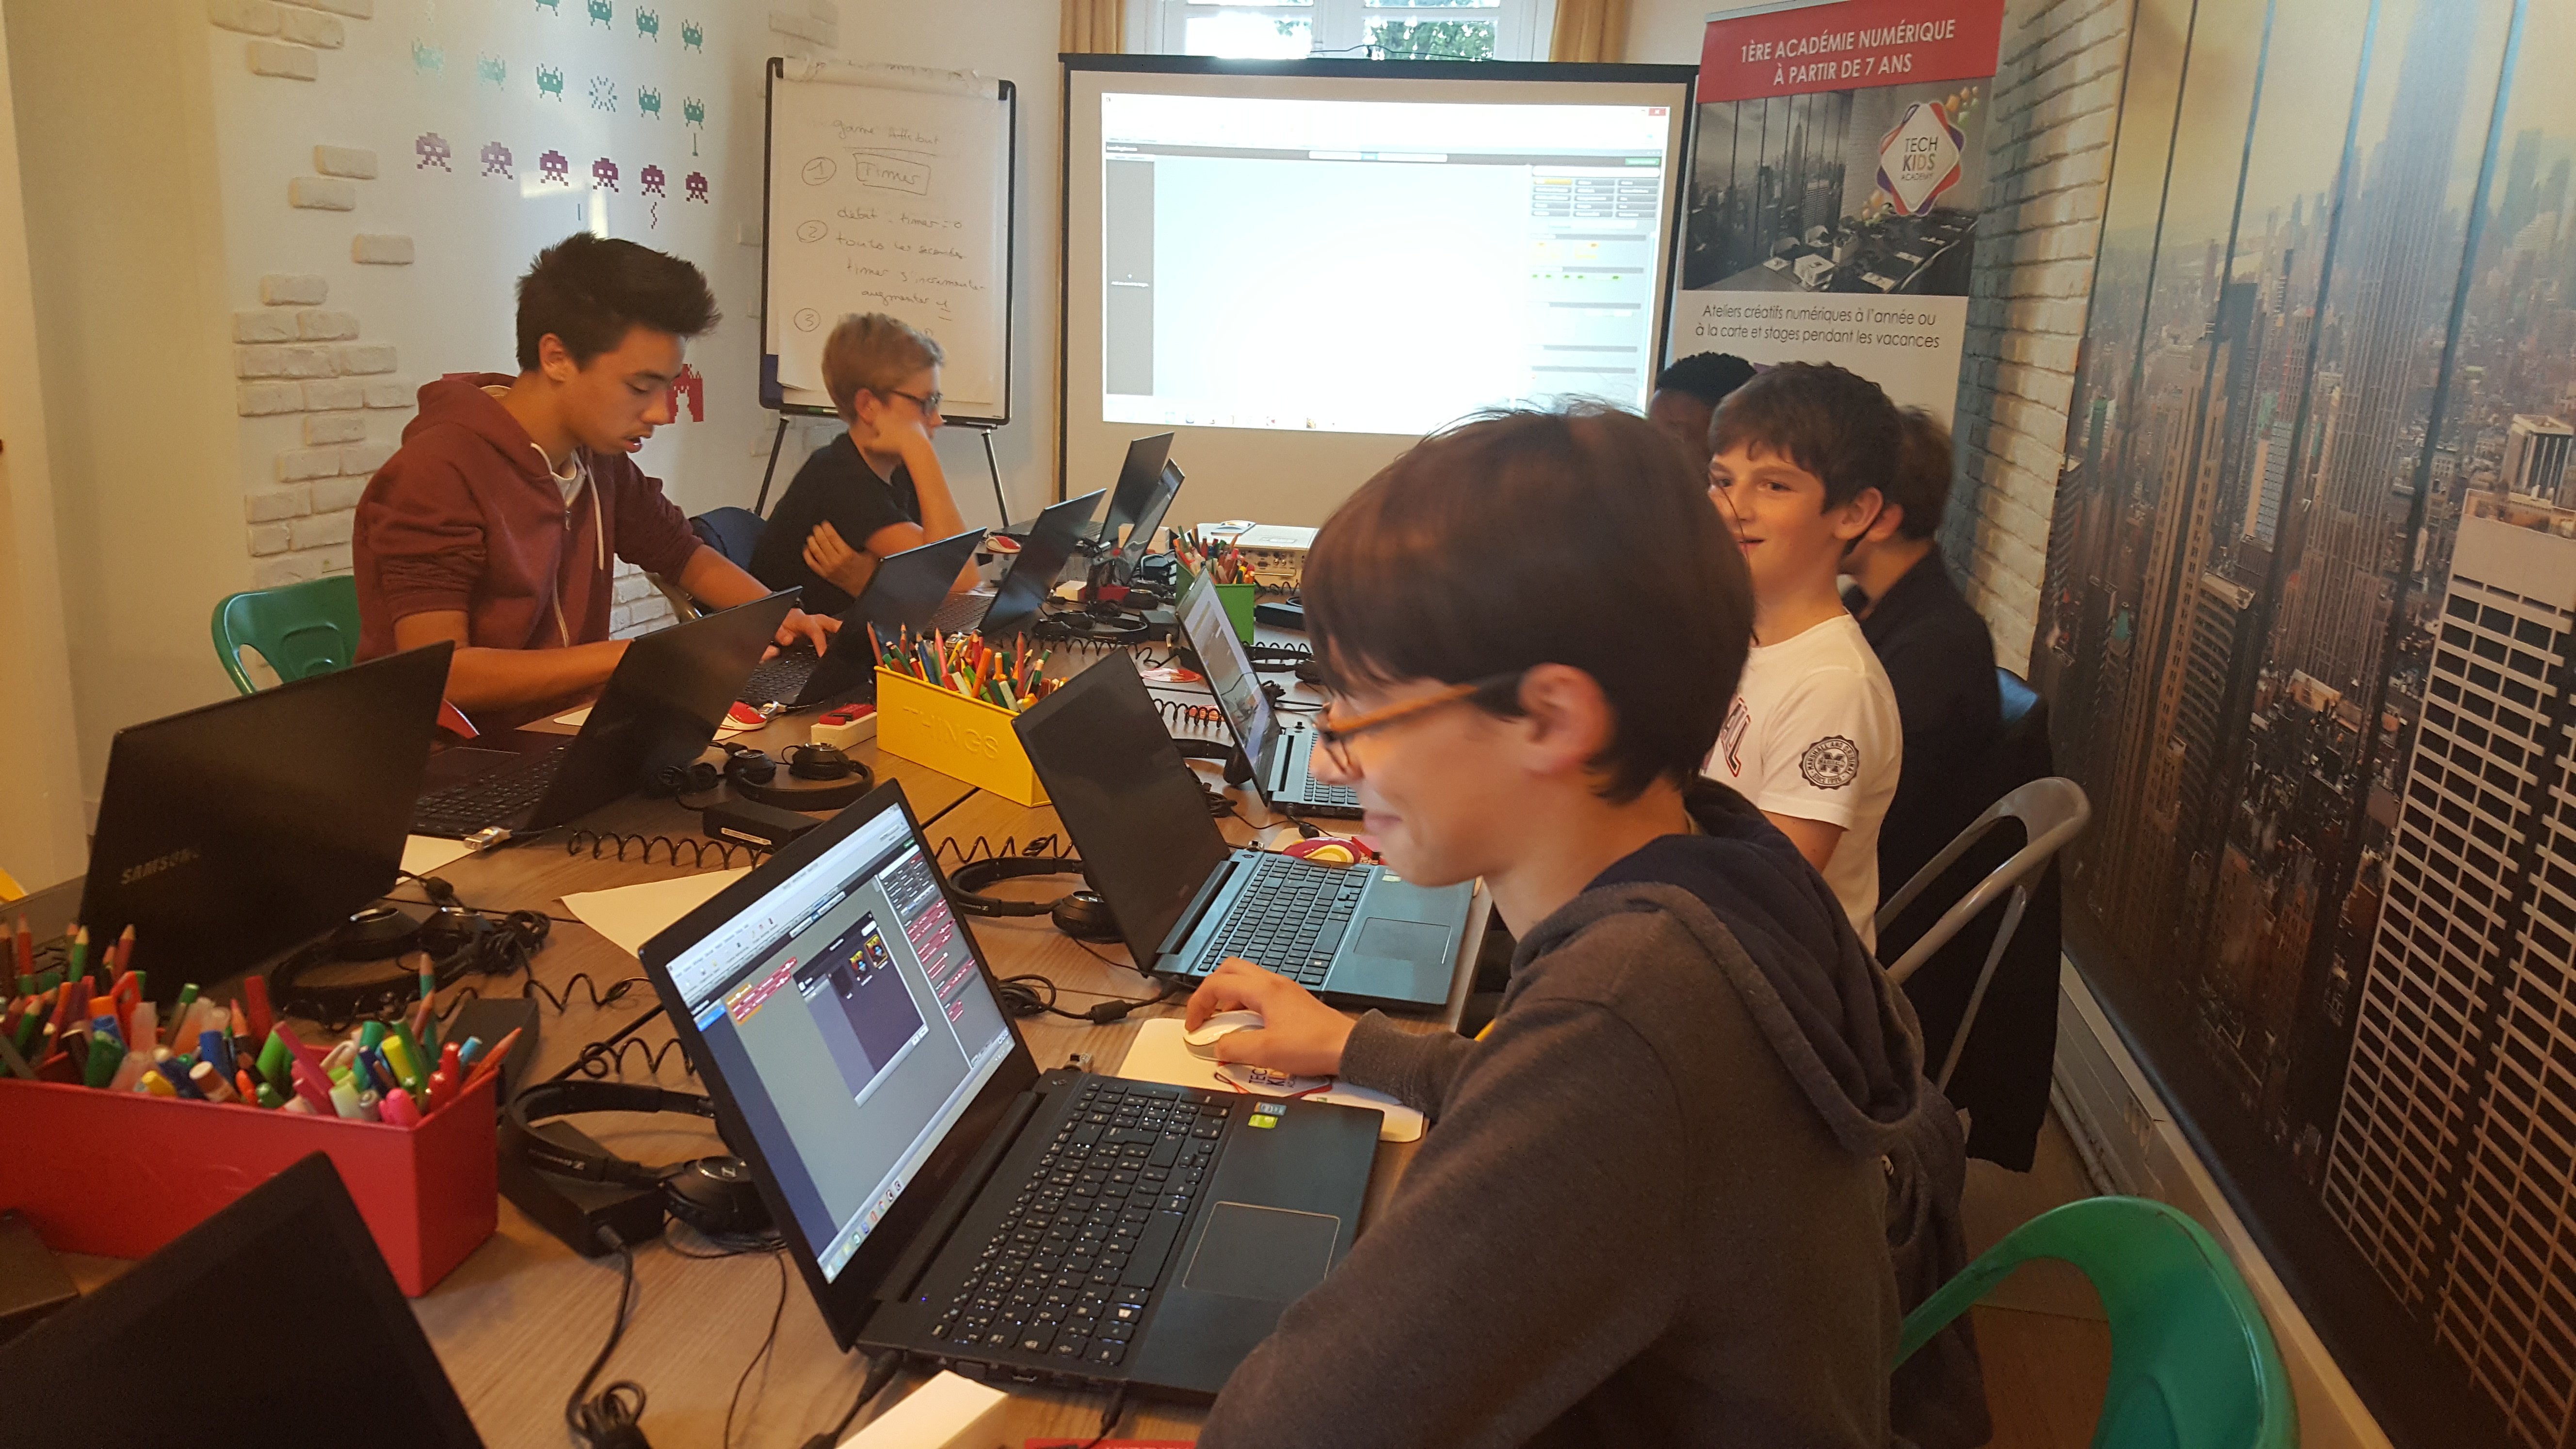
\includegraphics[width=73mm,scale=0.5]{images/techkidacademy.jpg}
%  \caption{Salle de classe Tech Academy}
%  \label{fig:boat1}
%\end{figure}

\newpage

\subsection{Apprendre à la "dure" ?}

Une autre solution est de tout simplement apprendre un langage de programmation avec des tutoriels disponibles sur internet. Il existe des sites spécialisés qui proposent l'apprentissage avec absolument aucune base informatique. C'est par exemple le cas de OpenClassroom (ex siteduzero). \cite{47} C'est personnellement sur ce site que j'ai commencé à me familiariser au langage C et aux principes de programmation durant mon lycée en autodidacte.

Néanmoins, bien que OpenClassroom développe des tutoriels assez bien expliqués et propose même un suivi sur son site sur l'évolution de son apprentissage, apprendre de cette façon implique plusieurs choses. Le public de ce genre de site est le plus souvent des étudiants ou même des professionnels en reconversion. Pour les autres qui seraient mineurs, ces derniers sont plus généralement des petits curieux cherchant à comprendre comment marche la programmation. Le bon point est que le site propose énormément de tutoriels et aujourd'hui certaines thématiques du site sortent même de l'informatique depuis l'internationalisation de ce dernier. L'utilisateur, si il n'a pas d'obligation peut s'orienter vers le langage qu'il souhaite découvrir. Les adolescents qui utilisent ce genre de site pour découvrir la programmation sont donc une minorité dans la population, cela prouve aussi qu'en utilisant cette solution ils sont motivés à apprendre ce domaine. Or, dans les exemples précédents de sensibilisation les enfants n'avaient parfois aucune idée de ce qu'était la programmation et les techniques servaient notamment à leur présenter le domaine et à se donner une idée de si ça peut leur plaire. Dans le cas de OpenClassRoom, nous avons un public déjà convaincu. Ces derniers ont une volonté d'apprendre, dans les exemple précédents on 'camoufle' l'apprentissage avec des moyens dérobés comme les jeux, l'interaction graphique etc... 

Par conséquent, il n'y a pas vraiment d'esprit ludique dans ces solutions mais par contre on va tout de suite dans la profondeur des choses. Si on est très motivé pour apprendre un langage on peut passer par ce genre de site. Toutefois, aucune équipe enseignante va suivre l'évolution de l'utilisateur en direct. Openclassroom propose cependant des systèmes de tuteurs mais c'est bien évidemment payant.

Un risque de ce genre de solution est aussi que la programmation peut devenir intimidante  voire même engendrer un mauvais ressentis si on baisse trop vite les bras. Même si le site fait en sorte de progresser dans le langage doucement, il nécessite quand même une grande attention pour certains chapitres et un investissement. L'apprentissage est en plus fait pendant le temps libre contrairement à d'autres solutions présentées qui se faisaient en classe ou dans une activité extra-scolaire.

Ce qu'on peut tout de même noter c'est que par exemple Openclassroom utilise le MOOC (massive open online course) traduit par formation en ligne ouverte à tous ou des professionnels et/ou spécialistes du domaine partagent donc leur savoir en vidéo accessible à tous. Ce genre de solutions donnent de bons résultats dans l'enseignement. \cite{48}

\newpage

\subsection{Solutions nécessitant des bases informatiques}

En ouverture de cet état de l'art, nous allons aborder quelques solutions ludiques qui nécessitent des compétences informatique. Cela montre que faire de l'informatique ludique n'est pas seulement pour les néophytes.

Nous pouvons parler dans un premier temps de Robocode, projet open source, \cite{49} qu'on peut classifier dans les serious game étant donné que son premier objectif est destiné à l'apprentissage de Java. Le but de ce jeu est de programmer les réactions d'un char miniatures afin de faire des combats contre d'autres chars d'autres joueurs (Voir figure 2.22). Ainsi, les joueurs vont créer une compétition entre eux pour faire la meilleure intelligence artificielle de char afin de battre l'autre joueur et anticiper au mieux ses réactions. C'est un projet distribué gratuitement et mis à jour régulièrement (dernière mise à jour datant de mai 2019). Les meilleurs joueurs ont notamment recours aux réseaux neuronaux et/ou aux statistiques dans leurs algorithmes. Robocode est notamment présent dans des compétitions à travers le monde en Inde, Irlande, Espagne ... La communauté est active sur les forums du jeu et sa documentation est disponible gratuitement.

Tout ces éléments font que Robocode est une solution qui possède des caractéristiques qui font qu'on a envie de continuer à jouer. Même si certains joueurs peuvent pousser la compétition plus loin que les autres, si l'on reste aux bases du projet il sert notamment à apprendre Java de façon divertissante. Robocode est notamment un moyen d'apprentissage par problème pour les chercheurs. \cite{50} Il en ressort aussi de cette recherche que les étudiants utilisant RoboCode développent des compétences d'analyse de code, de tests, d'implémentation ainsi que de l'esprit critique sur leur travail. Des exemples de robots sont disponibles sur le GitHub de RoboCode. \cite{51}

\begin{figure}[!htb]
  \centering
  \includegraphics[width=80mm,scale=0.5]{images/robocode.jpg}
  \caption{Un combat RoboCode}
  \label{fig:boat1}
\end{figure}

On peut également parler de TIS-100, un jeu vidéo disponible sur des plateformes de jeux comme Steam. C'est un jeu de type puzzle où le but est de réaliser des tâches sur un vieil ordinateur des années 70 en assembleur. Même si cela n'est pas exactement de l'assembleur mais une copie, on retrouve quand même la complexité de travailler avec des langages de bas niveaux. Pour expliquer le jeu plus clairement, nous avons une interface avec plusieurs blocs dont certains peuvent être corrompus, il faut alors ré-écrire ces blocs pour réparer la machine. Nous utilisons alors les registres de la machines ainsi que des commandes comme MOV, JEZ, SWP, ADD, JMP. (Voir annexe) Si nous n'avons jamais programmé en assembleur, c'est un bon moyen d'avoir une vision de son fonctionnement avec le jeu vidéo. \cite{52}

\newpage

\section{Critique de l'existant et solutions envisagées}

En conclusion de cet état de l'art, nous pouvons déjà faire une remarque sur l'existant : il est très vaste. Je ne m'attendais pas à trouver autant de sources avant de commencer ce mémoire. Depuis 1967, avec Logo, différents projets ont émergé avec l'objectif d'apprendre aux enfants l'informatique de façon ludique. Avec les technologies actuelles, des logiciels très complets permettent également de faire avancer la recherche (comme avec Scratch par exemple et sa fonctionnalité de statistiques d'utilisation de briques). Cependant, on observe que malgré la présence de projets de laboratoire de recherches il émerge aussi des projets commerciaux comme avec les serious game ou bien les activités de loisir informatique. Chacune ont leurs avantages et inconvénients (gratuit, payant, suivi, addicitif, pédagogique, complet ...). Les solutions comme Logo sont très complètes étant donné que l'interface de programmation est un éditeur de texte. Nous ne sommes soumis à aucune interface graphique même si on crée du graphisme avec la tortue, les possibilités avec les primitives de Logo sont importantes. Dans les système drag-and-drop l'interface et les briques de code sont définies, certes,  cela n'empêche pas la créativité mais le cadre est plus restrictif. Cependant ces cadres restrictifs font que l'enfant est plus accompagné et qu'il peut être plus attentif aux cours et ainsi mieux apprendre. Il y a aussi des environnements moins clairs pour les enfants que d'autres. Finalement on peut toujours trouver des défauts et des avantages, l'important est que l'existant est important et que par conséquent il est plus facile de trouver un équilibre entre tous ces points dans une solution qui nous correspond.

Une remarque que l'on peut faire est que depuis des années les chercheurs et les entreprises ont créé des solutions pour enseigner l'informatique aux enfants. Par conséquent, pourquoi ce n'est pas ou en tout cas très peu (Voir Zenika et Scratch) abordé en France ? Comme déjà évoqué en début de mémoire, en France l'éducation nationale préfère peut être se focaliser pour ce qui est de l'école primaire des matières fondamentales comme la lecture et l'écriture qui est parfois non acquise même en fin de cycle. Cependant, nous avons déjà vu que l'informatique est un domaine intéressant tant il apprend à percevoir le monde, et nous permet de réfléchir d'une autre façon. \cite{53} Avec l'existant, pourquoi ne pas tenter un enseignement dans les collèges lycée ? Nous avons nous même vu que la formation des professeurs pour certaines solutions n'était pas importante (cela ne nécessite pas des compétences haute d'informatique mais plutôt de la logique).

Les solutions proposées, malgré leurs interfaces destinées à des enfants, comprenaient souvent des problèmes de compréhension de la part de l'enfant. Ce n'est pas forcément par rapport au logiciel en lui même mais par rapport aux instructions et leurs agencement (On a notamment observé cela en Logo ou avec Scratch et la compréhension des briques). On peut alors penser qu'un environnement déjà familier à l'enfant peut lui permettre d'encore mieux appréhender les concepts.

En conséquence des observations précédentes, nous allons penser à des solutions très simple d'accessibilité car elles se rattacheront à des connaissances de l'enfant ou seront dans un univers ludique. Ainsi elles seront transposables directement sans avoir à faire des installations compliquées. Si c'est un univers déjà connu pour l'enfant cela attisera sa curiosité et renforcera sa motivation. 

\newpage

%%% Local Variables: 
%%% mode: latex
%%% TeX-master: "isae-report-template"
%%% End: 
\chapter{Apport}

\section{Introduction}

Il existe donc plusieurs possibilités pour appréhender l'informatique d'une façon divertissante, ludique et éducative. L'objectif de l'apport va être de proposer des idées dans ce sens et de également voir comment cela pourrait être implémenté. Est-ce que ces solutions sont implémentables en classe ? Quelles concepts sont abordés ? Est-ce que cela permet une réflexion personnelle de l'élève ? Comment amener l'élève à réfléchir d'un point de vue informatique au problème auquel il a été confronté ? Quel programme éducatif peut-on créer à partir de ces idées ?

Il me parait aussi très important que les solutions permettent l'interaction et qu'elles soient proche d'un environnement familier. En effet, cela permet d'améliorer l'implication de l'élève individuellement ou en groupe.

La possibilité d'accomplir des choses, de créer et de voir les résultats de sa création sont des sujets qui motivent l'élève, observations que nous avons notamment faites lors de l'état de l'art. Plus c'est visuel, plus l'élève est impliqué (en tout cas pour une initiation). Ainsi il me semble important de jouer sur ces facteurs. Si on arrive à faire quelque chose de visuel et dans un environnement familier on peut imaginer que cela peut amener à de meilleurs résultats.

L'apport n'a pas pour objectif de proposer des idées infaillibles et dont le résultat pédagogique est certain. Ce ne sont que des théories de ce qui pourrait être intéressant à mes yeux dans la pédagogie de concepts informatiques. On revient donc au point de départ avec la problématique du mémoire mais en ayant une idée de l'existant, cela va nous permettre de faire des remarques cohérentes sur les prises de décisions faites sur les solutions.

Le but est également de couvrir le maximum de concepts informatiques possibles, dans l'état de l'art nous avons pu voir que c'est surtout des concepts algorithmiques et de programmation qui étaient abordés. Ici, nous allons essayer, malgré le fait que l'on s'adresse à des enfants, d'aborder des notions variées et voir si elles sont transposables dans un programme d'éducation ou non. Même si elles ne sont pas complètes, nous proposerons au moins des ouvertures pour aller plus loin. Si certaines solutions hypothétiques peuvent se montrer non réalisables dans notre réalité (droits d'auteurs etc ...), on proposera alors une adaptation possible.

Concernant les critères de comparaisons nous utiliserons les mêmes que pour l'état de l'art, cependant nous ferons également en conclusion une comparaison de l'apport et de l'état de l'art concernant ces dits critères. Nous nous attarderons sur les différences entre les deux parties, pourquoi ces choix, avec un regard objectif sur l'apport et sa mise en oeuvre éventuelle dans la réalité.

\newpage

\section{Les solutions envisagées}

\subsection{Le Rubik's Cube, une énigme algorithmique}

Tout le monde connaît le Rubik's cube, ce casse-tête inventé dans les années 70. Casse tête géométrique en 3 dimensions, il est composé à l'extérieur de 26 cubes dont les faces peuvent se déplacer de droite à gauche (Voir figure). Si tout le monde connaît le rubik's cube, tout le monde ne sait pas le résoudre. On peut même être jaloux de ceux qui connaissent les systèmes de résolution du Rubik's Cube étant donné que l'on peut essayer de le résoudre pendant des heures sans y parvenir.

\begin{figure}[!htb]
  \centering
  \includegraphics[width=30mm,scale=0.5]{images/rubiks-cube.png}
  \caption{Un Rubik's cube}
  \label{fig:boat1}
\end{figure}

Le Rubik's cube est donc composé de 26 cubes et 6 faces. Chaque cube a sa propriété : pièce centrale, pièce arête et pièce de bord. La pièce centrale est de une couleur, la pièce arête de deux couleurs et la pièce de bord de 3 couleurs. Les pièces centrales sont fixes, la blanche est toujours en face de la jaune, la rouge est toujours en face de la orange et la bleu est toujours en face de la verte. Les autres pièces tournent donc autour des centrales. Si nous modifions le cube en le mélangeant le but est donc de remettre en ordre les faces (c'est à dire une face, une couleur).

Maintenant, comment allons nous introduire les concepts d'algorithmes sur le Rubik's cube ? Avant toute chose, il faut définir les variables auxquelles nous allons exécuter des instructions. Tenons notre Rubik's cube de face et nous aurons donc une face avant, haut, droite et gauche. Ainsi à partir de là nous pouvons définir pour chaque face une variable. Par exemple h pour haut, d pour droite, g pour gauche, a pour avant, et b pour bas. Inutile de définir une variable pour la face arrière car nous n'en aurons pas l'utilité lors de la résolution du cube et l'utilisation d'algorithmes. Maintenant si on s'attarde aux mouvements possible du Rubik's cube, on peut affilier des instructions à ses variables. Quels sont les mouvements possibles si l'on a un rubik's cube de face ? On peut tourner 'a' vers la droite ou la gauche, 'd' en avant ou en arrière etc... Par conséquent, on peut définir a+ pour tourner la face avant dans le sens des aiguilles d'une montre et a- pour le sens contraire des aiguilles d'une montre. Par exemple, exécuter la commande 'tourner la face avant vers la droite' on l'a traduit alors par 'a+'. On peut ainsi définir un algorithme comme 'a+ b+ d-' sois trois instructions tourner la face avant à droite, la face bas en avant et la face de droite en avant (sens contraire aiguille d'une montre). Ce qu'il faut retenir c'est que '+' signifie qu'on est toujours dans le sens des aiguilles d'une montre pour une face. Il suffit alors de tourner le cube vers cette face pour être bien sur de son instruction (est-ce que je tourne bien dans le sens horaire?). Nous pouvons aussi introduire une instruction 'h2' comme 'tourner 2 fois la face du haut'.

Malgré le fait que l'on tourne le cube il faut toujours garder les même références c'est à dire que la face avant ne change pas lors du déroulement d'un algorithme et que, après une instruction, il faut toujours repartir de ce point de référence. Il faut donc par exemple se mettre en face de la face avant. Bien évidemment, ce que j'explique plus haut est bien plus clair lorsqu'on le fait avec un Rubik's cube entre les mains.

\newpage

Maintenant que nous avons expliqué brièvement comment on pouvait implémenter des variables et des algorithmes sur le Rubik's cube nous pouvons donner un exemple concret. Le Rubik's cube se résout en une multitude d'étape que l'on peut séparer facilement. La première étape de la résolution du Rubik's cube étant assez triviale il n'y a pas vraiment d'algorithme, il suffit d'avoir ce que l'on appelle la croix blanche (Voir figure). Si l'on est novice au Rubik's cube, cette étape sert notamment d'introduction aux mouvements du Rubik's cube et permet aussi une introduction à la visualisation dans l'espace, un autre point intéressant.

\begin{figure}[!htb]
  \centering
  \includegraphics[width=60mm,scale=0.5]{images/rubiks-cube2.PNG}
  \caption{La croix blanche}
  \label{fig:boat1}
\end{figure}

Comme dit précédemment, comme cette étape est plutôt triviale il n'y pas vraiment d'algorithme, cependant il peut exister quelques cas particulier où l'on peut en appliquer. \cite{54}

Une fois qu'on a atteint cette étape,il faut remplir la face blanche. C'est un premier exemple d'utilisation d'algorithme dans le Rubik's cube. Comme on peut le voir dans la figure ci dessus, il reste alors 4 cubes contenant une face blanche. Nous allons les placer sous la position sur lesquels ils doivent être (donc sur la face du bas) et appliquer un algorithme. En partant donc de la référence croix sur la face du haut on applique : d- b- d+ b+. Bien sur dans ce cas la face dont la position doit être modifiée est en bas à droite par rapport à notre référence. Ce que l'on peut notamment observer sur cet algorithme c'est qu'il peut ne pas fonctionner du premier coup. En fait, dans ce cas il faut le boucler jusqu'à ce qu'il marche, pour expliquer cela dépend de l'orientation de départ de la face blanche sur le petit cube.

\begin{figure}[!htb]
  \centering
  \includegraphics[width=60mm,scale=0.5]{images/rubiks-cube3.PNG}
  \caption{Face blanche complète}
  \label{fig:boat1}
\end{figure}

Ce qui est intéressant à partir de cette étape c'est que toutes les suivantes découlent d'autres algorithmes. Ces derniers sont relatifs aux cas particuliers sur lesquels on peut tomber. L'étape suivante consiste à faire ce qu'on appelle la deuxième couronne (voir annexe). Nous avons alors les deux premiers étages de la bonne couleur. Nous n'allons pas expliquer en détail la résolution du Rubik's cube ici, même si dans l'annexe sont définis tous les algorithmes pour tous les cas possibles et pour toutes les étapes. L'idée à travers cette partie était de montrer le lien entre le Rubik's cube et l'algorithmique.

\newpage

Quel lien peut-on faire avec l'éducation et pourquoi utiliser cet outil ? Une première chose importante à prendre en compte c'est que le Rubik's cube est connu et que le désir de le résoudre vient naturellement à nous. Même sans savoir le faire, en ayant un Rubik's cube dans les mains de par la popularité du casse-tête on tend forcément à faire des tentatives. Par conséquent, inculquer ce désir est déjà réussi et on part donc d'un bon début. Il est donc peu utile, même si on le refera quand même comme un rappel, d'expliquer les bases du Rubik's Cube. Dans tous les cas, cela sera simple chez les élèves. Étant donné sa popularité, il sera également gratifiant de savoir le résoudre ce qui rajoute une motivation. Au vu du nombre de personnes qui savent résoudre un Rubik's Cube, savoir le faire est une sorte de 'super pouvoir' qui peut le pousser à montrer ses capacités et le motiver encore plus.

D'un point de vue pédagogique, l'apprentissage de l'algorithme est présent. Les idées d'instructions, variable, suite d'instructions pour résoudre un problème se conceptualisent dans un environnement très concret. Par conséquent l'enfant peut comprendre 1) ce qu'est un algorithme, les instructions, les variables et 2) son utilité donc ici résoudre un problème qui peut être une étape ou le Rubik's Cube tout entier.

Si nous voulons apprendre le Rubik's Cube à des enfants il faut les accompagner en leurs faisant des cours. De plus, le concept de Rubik's Cube ne peut pas être appris à de très jeunes enfants (au moins fin primaire ou début collège). Pour les jeunes enfants, ils risquent de s'y perdre dans toutes les étapes qui existent dans la résolution du Rubik's Cube. Par conséquent si l'on doit faire un curriculum sur un cours sur le Rubik's Cube, il faudrait dans un premier temps enseigner les propriétés de ce dernier (les faces, les cubes, les couleurs, les règles, les orientations, les points de références, les types de cubes (arête, coin, centre)). Ensuite un cours sur l'explication des algorithmes avec le Rubik's cube puis des cours d'apprentissage de résolution de problème avec les algorithmes pour différentes étapes. Il peut aussi être intéressant d'expliquer pourquoi ces algorithmes fonctionnent. Il est également important de faire un cours récapitulatif sur les notions vues pour avoir une idée de la compréhension du problème et du sujet par les élèves. 

Cet apprentissage rejoint le concept d'apprentissage manuel vu notamment avec le CS Unplugged, on peut je pense réintégrer certains avantages connus de ce programme dans cette solution car encore une fois on apprend sans ordinateur. Également, en plus de l'informatique on peut rattacher à ce genre de cours à des problèmes de géométries étant donné qu'on doit souvent voir les problèmes dans l'espace pour les enfants. D'un point vue logistique, les rubik's cube sont très accessibles et facilement transposables dans une salle de classe.

Enfin, on peut faire une critique sur cette solution, en effet au vu des étapes différentes on peut penser que la complexité pour un enfant peut être rebutante, on peut s'y perdre facilement et l'apprentissage d'algorithmes pour les étapes peut être répétitif, même si de toute façon le but n'est pas de devenir un as un Rubik's Cube mais d'appréhender des notions d'informatique de façon ludique. 

On peut également se demander si la résolution du Rubik's Cube est accessible aux enfants. Sachant qu'il existe des enfants de 7 ans qui arrivent à le résoudre en moins de 30 secondes et à une main \cite{55} on peut supposer qu'avec un bon accompagnement cela est tout a fait atteignable pour des enfants de 10 à 14ans.

Bien évidemment il faut tester cette solution sur des classes d'enfants et voir si il y a des adaptations à faire notamment avec les problèmes de mémorisation qui peuvent survenir (en raison de toutes les étapes de résolution). Mais ce qu'on peut conclure c'est qu'il y a des avantages mathématiques (vision spatiale du problème) et informatiques (algorithme).

\newpage

\subsection{Minecraft et la redstone}

Minecraft est l'un des jeux incontournable de notre époque et il est aussi très populaire chez les enfants. C'est un jeu de type bac à sable où le joueur intervient dans un monde où il peut le modifier à sa guise. La construction y est complètement libre et permet de développer son esprit créatif. De plus, le jeu propose un mode de survie avec un système de jour et nuit où il faut se cacher des monstres la nuit. Pour cela le jeu propose un système d'artisanat qui permet au joueur d'évoluer dans ce monde virtuel. Tout est cube dans le jeu, chaque ressource est un cube et les constructions se font également cube par cube.

C'est un jeu extrêmement populaire, c'est même devenu récemment le jeu le plus vendu de tous les temps dépassant Tetris avec 176 millions d'exemplaires. \cite{56} Par conséquent il est une référence pour beaucoup d'enfants et cela en fait un environnement parfait pour l'apprentissage, en effet les enfants ont alors l'impression de jouer alors qu'ils apprennent. C'est notamment ce qu'à fait le site code.org qui propose des serious game pour les enfants. Parmis ces serious game existe un jeu inspiré de Minecraft. Ici c'est sous la forme d'un jeu drag-and-drop comme on a déjà vu précédemment dans l'état de l'art. \cite{57}

Ce qui nous intéresse dans Minecraft ce n'est pas le jeu à proprement parler mais une des fonctionnalité du jeu : la Redstone. C'est un élément du jeu qui sert de fil conducteur entre différents blocs. C'est à dire que l'on peut lier des blocs entre eux avec un fil conducteur (la redstone) et créer des systèmes logiques (la porte s'ouvre quand j'appuie sur le bouton).

La Redstone était initialement prévue pour augmenter la distance d'action d'un levier ou d'un bouton pour activer des objets mécaniques comme un piston, une porte etc. Aujourd'hui la redstone suit les logiques implémentées dans les circuits (comme les porte logique, OR, XOR, NOR, AND). Cette fonctionnalité permet donc de faire des circuits logique avec énormément de possibilités. Les plus acharnés on par exemple créé un calculateur de la suite de Fibonacci avec la Redstone. \cite{58} 

L'usage de la Redstone est simple même pour les nouveaux joueurs, dans un premier temps cela requiert juste de mettre un signal logique entre un actionneur et un déclencheur (voir la figure ci dessous). Le signal rouge visible sur le sol a une limite de 16 blocs qu'il faudra alors allonger avec un répéteur, un objet du jeu qui a de multiple propriétés dans les circuits (retardateur, alimentation, mémorisation).

\begin{figure}[!htb]
  \centering
  \includegraphics[width=75mm,scale=0.5]{images/minecraft.png}
  \caption{Activer un piston avec de la redstone et un levier}
  \label{fig:boat1}
\end{figure}

Partant de ce simple statut, les possibilités sont très grandes car on peut faire des systèmes autonomes utilisant les portes logiques, table de vérités etc. Il existe en fait énormément de blocs dans le jeu liés à la redstone qui permettent ces grandes possibilités. \cite{59} Ici, nous ne ferons pas d'explication détaillée sur la redstone et nous n'allons pas apprendre comment faire une calculatrice sur Minecraft (même si c'est possible). Nous allons plutôt voir comment implémenter les portes logiques.

\newpage

Avant d'expliquer les portes logique il faut introduire le système de torche de redstone, visible dans la citation précédente. Ces torches servent à faire passer le courant. Elles sont, par défaut, allumées, pour en éteindre une, il faut passer du courant dedans et ce courant passe par le bloc qui sert de socle à la torche. On peut voir ce fonctionnement dans les figures ci dessous.

\begin{figure}[!htb]
  \centering
  \begin{minipage}[b]{0.45\textwidth}
    \includegraphics[width=\textwidth]{images/minecraft2.png}
    \caption{Levier éteint, la torche est allumée (par défaut elle est)}
  \end{minipage}
  \hfill
  \begin{minipage}[b]{0.45\textwidth}
    \includegraphics[width=\textwidth]{images/minecraft3.png}
    \caption{Levier allumé, on passe le courant au bloc socle, la torche s'éteint}
  \end{minipage}
\end{figure}

Maintenant que ce système est compris, on peut implémenter avec la redstone l'opérateur booléen AND. C'est à dire qu'on va avoir deux leviers et c'est seulement quand les deux sont allumés qu'un piston va s'activer. Ce système est visible avec la figure ci dessous.

\begin{figure}[!htb]
  \centering
  \includegraphics[width=90mm,scale=0.5]{images/minecraft4.png}
  \caption{Implémentation de l'opérateur booléen AND, le panneau résume les états possibles des leviers}
  \label{fig:boat1}
\end{figure}

Dans l'image, nous avons le premier état écrit sur le panneau de la capture d'écran sois 0 0. En effet comme on peut le voir, aucun courant passe dans les signaux par terre (à droite), si on active un levier on sera dans le cas 0 1 ou 1 0 et par conséquent le piston ne va toujours pas s'activer. En effet il y aura toujours une des deux torches allumées sur les blocs ce qui fera que le courant sur le bloc centrale sera toujours actif. Dans le cas où l'on active les deux leviers, les deux torches sur les blocs vont s'éteindre, le courant qui passe entre ces deux blocs va s'éteindre également et étant donné qu'il n'y aura plus de courant qui passera dans le bloc socle central, la troisième torche s'allumera ce qui fera passer le courant dans le circuit à gauche et qui activera le piston. Ce système est bien plus compréhensible avec le jeu en face de nous car dans ce cas on peut interagir, et mieux comprendre les différentes propriétés des blocs. On peut préciser que dans notre exemple nous avons deux entrées mais il est possible de faire des systèmes à 4, 8 ou 16 entrées.

On peut également parler de l'opérateur logique OR, encore plus simple d'implémentation, si nous prenons un cas à deux entrées comme l'exemple précédent, il suffit alors d'activer seulement un des deux leviers pour activer le piston. Cette exemple est visible dans la figure ci dessous.

\newpage

\begin{figure}[!htb]
  \centering
  \includegraphics[width=100mm,scale=0.5]{images/minecraft5.png}
  \caption{Opérateur OR, dans le cas 1 0}
  \label{fig:boat1}
\end{figure}

Dans cette figure on observe que l'on a activé le levier de gauche et non celui de droite et cela active quand même le piston. Un seul levier activé fait passer le courant ici. Nous pouvons implémenter d'autres opérateurs logiques comme le NAND, NOR, XOR, XNOR mais nous n'allons pas ici tous les définir. Certains autres exemples sont cependant disponibles en annexe.

Les opérateurs booléens ne sont pas les seules possibilités avec Minecraft, ici nous abordons vraiment les bases de ce que l'on peut faire avec la Restone. Il existe aussi la possibilité de faire des mises en mémoire tampon et des systèmes complexes (comme par exemple certains joueurs qui ont fait une calculette avec la Redstone \cite{60}) Nous n'allons pas tout aborder ici mais cela montre que les possibilités de problèmes logiques et algorithmiques que nous pouvons créer sont très grands. Étant donné que Minecraft est un jeu de construction composé de blocs qui fait que tout le terrain est modifiable les limites sont presque infinies.

Quel rapport peut-on faire entre ces faits et l'éducation ? Comme dit précédemment Minecraft est un jeu très populaire et par conséquent le fait que les élèves soient impliqués dans des exercices en rapport avec Minecraft augmente les chances d'attention de ces derniers. Ensuite, les exercices avec la Redstone permettent à l'enfant d'entrevoir les notions d'entrées sorties, de binaire, comment marche un circuit électronique, les opérateurs booléens et par conséquent des notions algorithmiques.

Si l'on veut transposer Minecraft dans un programme éducatif on pourrait par exemple réfléchir à des cours d'initiation à la redstone et à son fonctionnement, d'initiation aux opérateurs booléens et d'exercices pratiques impliquant la redstone (imaginons par exemple, faire un système de mots de passe à 5 leviers pour ouvrir la porte de sa maison). Cependant, il ne faut pas oublier que Minecraft est un jeu vidéo et que par conséquent l'élève risque de tenter de vraiment jouer au jeu plutôt que de se focaliser sur la redstone. Pour cela, il faudrait mettre en place une structure restrictive qui ne permet pas d'accéder aux fonctionnalités du jeu (survie, exploration etc...) mais qui se focalise sur la redstone et sur la créativité. Imaginons par exemple une carte vierge où l'on a les blocs strictement nécessaire à l'exercice. 

Enfin, le jeu est payant ( \EUR{23,95}) et par conséquent le mettre en place dans les écoles impliquerait d'acheter des licences ce qui peut être parfois rébarbatif quand on propose une solution encore jamais explorée et dont les résultats pédagogiques sont incertains.

\newpage

\subsection{World Of Warcraft pour apprendre le SQL ?}

Comme Minecraft, World Of Warcraft est un jeu très populaire. Cependant, contrairement à Minecraft il est très complexe. C'est un jeu en ligne multijoueur qui se déroule dans un univers fantastique. Deux factions se combattent et chaque faction possède ses différentes races de personnages. Un personnage dans le jeu appartient à une classe (mage, guerrier, prêtre ...). Chaque classe à des sorts, compétences, spécialisations. Le personnage progresse dans un monde virtuel où il navigue entre différentes zones du jeu, rencontre d'autres personnages (joueur et non joueur) et participe à des quêtes, ramasse des objets etc... Cette complexité dans l'univers de World Of Warcraft fait que toutes ces données doivent être rangées dans une base de données et que des liens doivent être faits entre les différentes tables de la base.

Lorsque j'ai personnellement voulu essayer de faire un serveur World Of Warcraft dans sa version Vanilla (donc sans extension), j'ai utilisé un système qui s'appelle MaNGOS. \cite{61} \cite{62} Par exemple pour World Of Warcraft Vanilla, il partage un serveur, une base de données et les scripts pour le jeu. Une fois toute l'installation faite, nous avons donc accès à cette base de données qu'il faut de toute façon obligatoirement modifier pour mettre en place le serveur.

MaNGOS propose en faite une base de données calquée sur le modèle de World Of Warcraft (donc recréée) avec sa documentation complète. \cite{63} Il y a plus précisément deux bases de données "mangos" pour le jeu et "realmd" pour tout ce qui est compte et serveur. Faisons par exemple un 'SHOW TABLES' sur realmd on obtient le tableau suivant.

\begin{table}[!htb]
\centering
\begin{tabular}{|l|}
\hline
Tables\_in\_realmd    \\ \hline
account               \\
account\_access       \\
account\_banned       \\
antispam\_blacklist   \\
antispam\_detected    \\
antispam\_replacement \\
antispam\_unicode     \\
ip2nation             \\
ip2nationcountries    \\
ip\_banned            \\
migrations            \\
realmcharacters       \\
realmlist             \\
uptime                \\ \hline
\end{tabular}
\end{table}

Si par exemple nous faisons un 'SELECT * FROM account' nous aurons la liste des comptes suivant ce schéma \cite{64} et si nous faisons 'SELECT * FROM realmlist' nous aurons la liste des serveurs suivant ce schéma. \cite{65}

Ce qui est maintenant intéressant c'est qu'une action sur ces tables entraînera alors le fait que l'on peut par exemple se connecter avec un nouveau compte sur le jeu (si l'on a fait un INSERT INTO d'un n-uplet) ou qu'on ne peut par exemple plus se connecter sur un compte (si l'on a fait un DELETE sur une ligne). Il en va de même pour les serveurs.

Pour l'autre base de données, en plus de pouvoir effectuer des actions similaires (retrait de sort, ajout d'un personnage non joueur...). On utilise en plus le système de clé primaire pour faire le lien entre les tables. Imaginons que nous voulons créer une creature suivant ce modèle :

\begin{lstlisting}[frame=single]
(guid, id, map, modelid, equipment_id, position_x, position_y, 
position_z, curhealth, curmana, DeathState, MovementType)
\end{lstlisting}

Il faut alors faire référence à un modelid qui suit ce modèle 
\begin{lstlisting}[frame=single]
(modelid, bounding_radius, combat_reach, gender)
\end{lstlisting}

Ainsi après avoir inséré notre créature avec ses paramètres et sa position il sera directement visible dans le jeu. C'est ici que c'est ludique, car nos actions dans la base de données font que le jeu est modifié et c'est visible directement. Il est alors amusant de voir toutes les possibilités que l'on a en changeant cette base de données (modifier la taille de certains personnage, changer les positions de départ des joueurs après avoir créé un personnage). Il est aussi très intéressant de voir comment marche une base de données dans un cas concret et les liens entre les classes. Si nous voulons voir ça d'un point de vue éducatif, il faudrait alors apprendre les structures d'une base de données et apprendre dans un premier temps comment on navigue dedans. Ensuite on pourra apprendre les commandes de base du SQL (SELECT, UPDATE, DELETE ...) et voir leurs effets directement dans le jeu.

Cependant, travailler avec la base de données MaNGOS est complètement inconcevable dans un cadre éducatif et ça pour plusieurs raisons. Dans un premier temps la base de données est très complexe et pas forcément évidente, certaines tables utilisent trop de données souvent incompréhensibles pour quelqu'un de non initié. Les noms de tables ne sont pas familiers, les paramètres sont incompréhensibles etc... Ensuite, aussi parce que World Of Warcraft appartient à une entreprise. Il est complètement illégal d'utiliser son logiciel de cette façon et cette base de données (MaNGOS) aussi. Le jeu n'est pas du tout adapté pour ce genre d'utilisation vu qu'il est utilisé pour le jeu en ligne. Enfin, World Of Warcraft est un jeu déconseillé pour les enfants.

Le point essentiel de MaNGOS et de sa base de données est que l'utilisation et la modification de cette dernière est divertissante tant on voit l'impact qu'elle a sur le jeu. On a alors envie de découvrir par nous même cette base et y appliquer des modifications pour créer toutes sortes de scènes, parfois surréalistes, parfois pour tricher dans le jeu tout simplement. C'est cet effet que ça a eu notamment sur moi qui me semble important pour le point de vue pédagogique. Comme pour Minecraft, on a l'impression de jouer en apprenant.

MaNGOS n'est au final qu'un prétexte. C'est pour faire comprendre qu'en réalisant un environnement fait pour l'apprentissage utilisant le SQL, on pourrait créer quelque chose de ludique autour de cette technologie. Imaginons maintenant une base de données semblable à MaNGOS mais sans sa complexité. C'est à dire que l'on garderait un univers fantastique comme World Of Warcraft (Race, classe, spécialité etc...) ou tout serait stocké dans une base de données. Ensuite une modification de cette base entraînerait une modification dans un univers virtuel semblable à World Of Warcraft. Par conséquent avec un tel système, on serait capable d'impliquer l'enfant dans une base de données et son fonctionnement grâce à l'environnement proposé. On pourrait alors lui apprendre à naviguer dans la base avec des noms de tables parlant (creature, personnage, sort, quête). Et lier ces tables entres elles (un n-uplet de quête lié à l'id d'un personnage) et pouvoir faire des modifications facilement dans cette dernière.

Si on veut créer un dispositif d'enseignement autour de cette idée, il faudrait dans un premier temps créer le logiciel et ensuite réfléchir aux exercices à faire dessus. L'important étant d'aborder des points comme : comment fonctionne les bases de données, comment naviguer dans une base de données, quels sont les commandes de bases d'une base de données et quels sont les effets de ces commandes.

\newpage

\subsection{Le cas Raspberry Pi}

Le Raspberry Pi est un micro-ordinateur au prix de vente faible (environ \EUR{25} ). Cela permet une bonne distribution du produit. Si l'on prend du recul on peut même dire que cela peut être une solution pour des pays en voie de développement qui ne peuvent pas avoir un accès facile aux ordinateurs dans un cadre éducatif. Raspebrry Pi est distribué en général sous Linux, ce système d'exploitation souvent mystérieux pour beaucoup de personnes. Ce qu'il faut savoir sur cet ordinateur c'est qu'il a pour but d'encourager ses utilisateurs à l'apprentissage de la programmation informatique. C'est ce qui est directement visible sur le site officiel. \cite{66}

Malgré cela, notamment en France, il n'existe pas vraiment de programme d'éducation comprenant le Raspberry Pi. Pourtant, étant sous Linux, il permettrait aux enfants de découvrir cet environnement et notamment les commandes Unix (par exemple se déplacer dans les fichiers de l'ordinateur sans passer par un explorateur de fichier graphique). Il serait notamment intéressant d'apprendre d'autres commandes Unix dans un environnement ludique. Imaginons par exemple créer un serveur Minecraft sur une raspberry en passant par la console. \cite{67} Ensuite, on pourrait expliquer comment modifier les fichiers de configuration depuis la console également (à la création d'un serveur Minecraft nous sommes obligés de modifier un fichier qui stipule qu'on accepte le terme EULA, soit passer une variable dans un fichier texte à 'true'). Il est aussi possible de faire un lien pédagogique avec des notions de réseau (Pourquoi je peux me connecter sur mon serveur Minecraft en 127.0.0.1 ? Qu'est-ce que le port 25565 sur mon serveur ? pourquoi les autres joueurs peuvent rejoindre mon serveur ? Qui est le client et qui est le serveur ?)

Rien qu'avec Minecraft, qui nous permet plus facilement de communiquer avec les enfants, il y a beaucoup de possibilités envisageables avec le Raspberry. Surtout que comme dit précédemment, ce dernier a une volonté à la base pédagogique, comme ce qui est énoncé sur le site : "\textit{A small and affordable computer that you can use to learn programming}" . C'est notamment ce qu'on observe directement en se baladant dans la barre de tâche.

\begin{figure}[!htb]
  \centering
  \includegraphics[width=60mm,scale=0.5]{images/raspberry.PNG}
  \caption{Barre de tâche sur raspberry}
  \label{fig:boat1}
\end{figure}

On observe notamment la présence de Scratch et Sonic Pi, logiciels éducatifs dont nous avons déjà parlé et donc pré-installé sur la raspberry. Cela permet de facilement envisager des cursus d'enseignements liés à la raspberry. De plus Sonic Pi possède une fonctionnalité qui le lie à Minecraft \cite{68}, on peut donc plus ou moins lier les idées vu précédemment et créer un enchaînement logique.

\newpage

\section{Synthèse sur l'apport}

Les idées proposées dans l'apport ont un point commun. Partir de quelque chose de connu, que ce soit intriguant ou amusant pour en faire un projet éducatif. Si l'on a un sujet parlant pour les élèves et qui en plus propose de leur apprendre des choses on a alors le ludique et la motivation en un. Par exemple pour le Rubik's Cube en plus de savoir déjà ce qu'est un Rubik's Cube l'élève peut désormais entrevoir comment le résoudre, ce qui est déjà amusant tout en apprenant les algorithmes. Il en est de même pour Minecraft, il y a en effet beaucoup de domaines sous-jacents que l'on peut lier à Minecraft (opérateurs logique, système de client-serveur, lien avec Sonic Pi). De base le principe de Minecraft est lié à la créativité. Nous avons vu d'ailleurs dans l'état de l'art que l'association de la créativité (sujet qui est de base important chez l'enfant) avec l'apprentissage donne de bons résultats. Ces outils nous permettent donc d'aller plus loin que cet existant en proposant en plus de cela un environnement connu.

Malheureusement, la plupart des solutions possèdent des points négatifs, déjà certaines ne sont tout simplement pas implémentables aujourd'hui (cas World Of Warcraft), et d'autres posent le soucis du manque de données quant aux résultats pédagogiques de la méthode. Cependant, étant donné que l'on arrive forcément à lier les idées à des concepts informatiques on peut facilement supposer que cela peut avoir un impact positif. Il faut cependant réfléchir sérieusement à un dispositif d'apprentissage avec ces idées (découper en leçon, quels concepts apprendre et à quel moment, faire un cours récapitulatif sur ce qu'ont appris les élèves etc...).

\newpage
\chapter{Conclusion}

L'informatique est à la portée de tous. Dès l'enfance des outils sont à notre disposition pour apprendre des fondements informatiques qui peuvent paraître pourtant aux premiers abords compliqués. Ces outils sont en plus très nombreux et ce depuis les années 60. On reste cependant déçu par le fait qu'avec toutes ces ressources il n'y a pas clairement de dispositifs éducatifs créés par l'éducation nationale en France, même si cela est en bonne voie pour 2019. On peut noter qu'il y tout de même une volonté d'introduction à à l'algorithmique avec Scratch. \cite{25}

Avoir des notions informatiques est essentiel aujourd'hui pour comprendre le monde. Agriculture, industrie, médecine, divertissement, commerce ... L'informatique est absolument présente partout. Pourtant, le constat que l'on fait est que malgré cette présence quasi exclusive au final la majorité des gens ne savent pas écrire une ligne de code. On ne dit pas que tout le monde doit savoir coder, mais il est tout de même important d'avoir un aperçu de cette discipline, même général.

Sensibiliser les enfants permet également d'appréhender ce domaine sans posséder de stéréotype. Il est facilement visualisable que l'informatique est un domaine où il y a une majorité d'hommes. Pourtant, sur certaines études par exemple sur Scratch, nous avons vu que les filles se débrouillaient en moyenne mieux que les garçons sur certains aspects de la programmation. Pourtant, ces dernières, même si elles en ont les capacités, sont moins présentes en informatique à l'université. Appréhender l'informatique dès le jeune âge permet de casser ces stéréotypes et voir directement si ce domaine nous plaît ou non.

D'un point de vue purement technique, il a aussi été démontré que être sensibilisé à l'informatique permet de développer des nouvelles façons de résonner et de résoudre des problèmes de telle façon que cela n'existe pas encore aujourd'hui dans l'éducation. On a même pu voir que des concepts comme la récursion ou la concurrence était abordable même pour les enfants. Ce qui est clairement une preuve que l'informatique est accessible aux enfants. C'est même accessible de façon ludique.

Pourtant à l'école l'informatique en France se résume pour l'instant à l'obtention du B2i (Brevet informatique et internet) qui est pour résumer la preuve que l'élève sait lire des caractéristiques d'un fichier sur un système en particulier (Windows). Or, la programmation par exemple est un langage qui est adaptable sur tout système d'exploitation et même sur les objets connectés, les puces électroniques etc...

Aussi, en se concentrant sur l'état de l'art et l'apport de ce mémoire, il apparaît que l'introduction de l'informatique à l'école (que ce soit au primaire, collège ou bien encore au lycée) est clairement envisageable. C'est d'ailleurs un projet de l'éducation nationale pour le lycée puisqu'en 2021 entrera en vigueur le nouveau bac et que dès la rentrée 2019 il y aura un enseignement commun SNT (Sciences numériques et technologie) en seconde général qui parlera d'internet et du web, d'objets connectés de photos numériques etc... \cite{69}

En conclusion, familiariser les concepts informatiques aux enfants est d'abord possible et ensuite important pour appréhender le monde de demain. Cela permet de développer de nouvelles compétences et de casser, dès le plus jeune âge, les stéréotypes sur ce domaine pour permettre qu'il soit accessible à tous.

"\textit{Everybody in this country should learn to program a computer because it teaches you how to think}"

-Steve Jobs


%\addcontentsline{toc}{chapter}{Annexe}
\chapter{Annexe}


\begin{figure}[!htb]
  \centering
  \includegraphics[width=150mm,scale=0.5]{initial_structure_env.PNG}
  \caption{Environnement de développement pour enfant, source : \cite{1}}
  \label{fig:boat1}
\end{figure}

\newpage

Tableau des primitives de Logo (Principales primitives de la tortue) :


\begin{table}[htb]
\begin{changemargin}{-3cm}{-3cm}
\begin{tabular}{|l|l|l|}
\hline
\multicolumn{1}{|c|}{Français} & Anglais            & Définition                                                                                         \\ \hline
AV n ou AVANCE n               & FD n ou Forward n  & La tortue avance de n pas                                                                          \\ \hline
RE n ou RECULE n               & BK n ou Back n     & La tortue recule de n pas                                                                          \\ \hline
TD n ou TOURNEDROITE n         & RT n ou RIGHT n    & La tortue tourne de n degrés d'angle vers la droite                                                \\ \hline
TG n ou TOURNEGAUCHE n         & LT n ou LEFT n     & La tortue tourne de n degrés d'angle vers la gauche                                                \\ \hline
LC ou LEVECRAYON               & PU or PENUP        & La tortue ne laisse pas de trace                                                                   \\ \hline
BC ou BAISSECRAYON             & PD or PENDOWN      & La tortue laisse sa trace (par défaut)                                                             \\ \hline
CT ou CACHETORTUE              & HT ou HIDETURTLE   & La tortue n'est plus visible sur l'écran graphique                                                 \\ \hline
MT ou MONTRETORTUE             & ST ou SHOWTURTLE   & La tortue est visible sur l'écran graphique                                                        \\ \hline
ENR ou ENROULE                 & WRAP               & Enroule l'écran graphique (valeur par défaut)                                                      \\ \hline
FEN                            & WINDOWS            & La tortue peut sortir du jardin et disparaître de l'écran graphique                                \\ \hline
CLOS                           & FENCE              & La tortue ne peut pas sortir du jardin                                                             \\ \hline
ORIGINE                        & HOME               & Retour au milieu du carré de salade                                                                \\ \hline
VE                             & CS ou CLEARSCREEN  & Efface toutes les traces et restaure l'état initial   \\ \hline
NETTOIE                        & CLEAN              & Efface toutes traces de l'écran graphique sans changer la position                    \\ \hline
VT                             & CT or CLEARTEXT    & Efface l'écran de commande                                                                         \\ \hline
FCC n                          & SETPC n            & Change la couleur du crayon, n est un entier positif                                               \\ \hline
FCFG n                         & SETBG n            & Change la couleur du fond, n est un entier positif                                                 \\ \hline
FCB n                          & *****              & Change la couleur des bords, n est un entier positif                                               \\ \hline
FCAP n                         & SETH ou SETHEADING & Fixe le cap de la tortue de manière absolue, selon l'angle de n degrés                             \\ \hline
FPOS {[}X Y{]}                 & SETPOS {[}X Y{]}   & Fixe la POSITION de la tortue avec une LISTE de 2 nombres entiers \\ \hline
CAP n                          & HEADING            & Retourne l'orientation de la tortue exprimée en degrés                                             \\ \hline
POSITION, POS                  & POS                & Retourne la position de la tortue en coordonnées cartésienn                                        \\ \hline
\end{tabular}
\end{changemargin}
\end{table}

\newpage 

Primitives Logo mathématiques :

\begin{table}[htb]
\begin{changemargin}{-3cm}{-3cm}
\begin{tabular}{|l|l|l|}
\hline
\multicolumn{1}{|c|}{Français} & Anglais         & Définition                                                            \\ \hline
n1 + n2                        & n1 + n2         & Addition de nombres réels - Ex : EC 45.124 + 11 ou EC (+ 45 10 78 23) \\ \hline
n1 - n2                        & n1 - n2         & Soustraction de nombres réels - Ex :EC 5 - 1.09                       \\ \hline
n1 * n2                        & n1 * n2         & Multiplication de nombres réels - Ex :EC 5 * 9                        \\ \hline
n1 / n2                        & n1 / n2         & Division de deux nombres réels - Ex :EC 45 / 9                        \\ \hline
SOMME n1 n2                    & SUM n1 n2       & Addition de nombres réels - Ex : EC SOMME 45 11                       \\ \hline
DIFF n1 n2                     & - n1 n2         & Soustraction de nombres réels - Ex :EC DIFF 5 1                       \\ \hline
PROD ou PRODUIT n1 n2          & PRODUCT n1 n2   & Multiplication de nombres réels - Ex :EC PROD 5 9.45                  \\ \hline
DIV n1 n2                      & QUOTIENT n1 n2  & Division de deux nombres réels - Ex :EC DIV 45 11                     \\ \hline
QUOTIENT n1 n2                 & QUOTIENT n1 n2  & Division de deux nombres réels - Ex :EC DIV 45 11                     \\ \hline
RESTE n1 n2                    & REMAINDER n1 n2 & Reste de la division                                                  \\ \hline
ENT n                          & INT n           & Renvoie la partie entière du nombre réel - Ex :EC ENT 55.75 -> 55      \\ \hline
ARRONDI n                      & ROUND n         & Arrondit un nombre réel - Ex :EC ARRONDI 55.75 -> 56                   \\ \hline
ABS n                          & ABS n           & Renvoie la valeur un nombre réel - Ex :EC ABS -55 -> 55                \\ \hline
HASARD n                       & RANDOM n        & Renvoie un nombre entier entre 0 et n-1                               \\ \hline
RC n ou racine n               & SQR n           & Renvoie la racine carré d'un nombre réel - Ex :EC RC 25 -> 5           \\ \hline
LOG n                          & LOG n           & Renvoie le logarithme naturel d'un réel                               \\ \hline
LOG10 n                        & LOG10 n         & Renvoie le logarithme de base 10 d'un réel                            \\ \hline
EXP n                          & EXP n           & Renvoie l'exponentielle d'un réel                                     \\ \hline
SIN n                          & SIN n           & Renvoie le sinus d'un réel n en degrés - Ex :SIN 30                   \\ \hline
COS n                          & COS n           & Renvoie le cosinus d'un réel n en degrés                              \\ \hline
TAN n                          & TAN n           & Renvoie la tangente d'un réel n en degrés                             \\ \hline
ATAN n                         & ATAN n          & Renvoie tangente d'arc d'un réel n en degrés                          \\ \hline
PI                             & PI              & 3.141592…                                                             \\ \hline
RADIANS n                      & RADIANS n       & Convertit un angle en radians n en degrés                             \\ \hline
DEGRES n                       & DEGRES n        & Convertit un angle en degrés n en radians                             \\ \hline
\end{tabular}
\end{changemargin}
\end{table}

\begin{figure}[!htb]
  \centering
  \includegraphics[width=105mm,scale=0.5]{images/sonic_pi_primitives.PNG}
  \caption{Exemples de fonctions de Sonic Pi, source : \cite{19}}
  \label{fig:boat1}
\end{figure}

\begin{lstlisting}[frame=single]

live_loop :beeps do
  start_note = ring(60, 62, 63, 62).tick
  my_chord = chord(start_note, :M7)
  play my_chord, release: 2
  16.times do
    play my_chord.choose, release: 0.25, amp: [0.75, 0.5, 0.25].choose
    sleep 0.125
  end
end

live_loop :drums do
  sample :loop_amen, beat_stretch: 2
  sleep 2
end

\end{lstlisting}

Exemple d'un programme Sonic Pi


\begin{figure}[!htb]
  \centering
  \includegraphics[height=80mm, width=150mm,scale=0.5]{images/codecombat3.PNG}
  \caption{Niveaux suivants de CodeCombat}
  \label{fig:boat1}
\end{figure}

\begin{figure}[!htb]
  \centering
  \includegraphics[width=150mm,scale=0.5]{images/tis-100.jpg}
  \caption{Interface TIS-100 et blocs de code}
  \label{fig:boat1}
\end{figure}

\begin{figure}[!htb]
  \centering
  \includegraphics[width=80mm,scale=0.5]{images/rubiks-cube4.PNG}
  \caption{La deuxième couronne}
  \label{fig:boat1}
\end{figure}

\newpage

 
\newpage
Tous les algorithmes pour les étapes du Rubik's cube

\begin{lstlisting}[frame=single]

//face blanche
côté : d- b- d+ b+

//deuxième couronne
mettre à gauche : h- g- h+ g+ h+ a+ h- a-
mettre à droite : h+ d+ h- d- h- a- h+ a+
inversion : d+ h+ d- h2 d+ h2 d- h+ a- h- a+ 

//côté jaune après 2eme couronne
j jaune (1 en haut 1 à gauche) : d- h- a- h+ a+ d+
barre à l'horizontal : a+ d+ h+ d- h- a-
point jaune : d- h- a- h+ a+ d+ puis a+ d+ h+ d- h- a-

croix en face bien placé (2 bonne en face) : d+ h2 d- h- d+ h- d- puis
d+ h2 d- h- d+ h- d- h-

côté bien placé (mauvaise en face et à droite): d+ h2 d- h- d+ h- d- h-

1 coin à la bonne place + sens aiguille monte (le bon à droite) :
g- h+ d+ h- g+ h+ d- h-
coin à la bonne place 1 + sens inverse aiguille (le bon à gauche) : 
d+ h- g- h+ d- h- g+ h+
aucun bien placé : g- h+ d+ h- g+ h+ d- h-

-------------
coin bonne position 

2 mal orienté côte à côté (2pieces meme couleur à droite) : 
d+ h2 d- h- d+ h- d- g- h2 g+ h+ g- h+ g+
4 mal orienté (pareil à droite) : 
d+ h2 d- h- d+ h- d- g- h2 g+ h+ g- h+ g+
2 diagonale : a+ avec le jaune en face puis meme formule

3 coins mal orientés avec le jaune à droite : 
pareil avec 2 mauvais à droite
3 coins mal orientés avec le jaune à gauche : pareil

\end{lstlisting}

\newpage

\begin{figure}[!htb]
  \centering
  \includegraphics[width=120mm,scale=0.5]{images/minecraft6.png}
  \caption{Opérateur NOR dans minecraft}
  \label{fig:boat1}
\end{figure}

\begin{figure}[!htb]
  \centering
  \includegraphics[width=120mm,scale=0.5]{images/minecraft7.png}
  \caption{Opérateur NAND dans minecraft}
  \label{fig:boat1}
\end{figure}



\printbibliography[heading=bibintoc]

\appendix

\end{document}